\documentclass[a4paper,12pt]{hitec}

\usepackage{amsmath,amsthm,amssymb}
\usepackage{mathtext}

\usepackage[T1,T2A]{fontenc}
\usepackage[utf8]{inputenc}
\usepackage[ukrainian,english]{babel}


%\usepackage[english]{babel}
\usepackage{times}
\usepackage{setspace}
%\usepackage{inputenc}
\usepackage{amssymb}
\usepackage{amsfonts}
\usepackage[pdftex]{graphicx}
\usepackage{subfig}
\usepackage{alltt}
\usepackage{moreverb}
\usepackage{float} % to be able to use [H] float placement for figures
%for more info on hyperref package see http://en.wikibooks.org/wiki/LaTeX/Packages/Hyperref
\usepackage[pdftex,colorlinks=true,linkcolor=blue]{hyperref}

\begin{document}
  \begin{titlepage}
\title{Trident Genesis Platform Architecture from Engineering Perspective}
\company{Fielden Management Services Pty. Ltd.}
\author{TG Team}
\date{Lviv-Melbourne, 2011}
\maketitle
\clearpage
  This article provides a high level overview of the motivation, principle approaches and core features of the Trident Genesis software platform.
  The main emphasis is made on architectural and technological innovations, which together define a unique technology for the development and reliability improvement of business oriented applications.

\clearpage
\tableofcontents
\clearpage

\end{titlepage}
  \section{Geo-zones}
Geo-zone visual representation can be used as the first example of GIS web component possibilities. Geo-zones represent simple geographical polygons that can ``guard'' machine movements and help to store intersection events. They can be used to determine whether machine is in the right place in particular time or whether the route is performing well.

In Transmirror project Geo-zones have been used to determine the count of performed route circles on a daily basis for route vehicles. It helps the manager to control the amount of vehicle fuel usage. It also give an ability to quickly analyse whether the driver is on time on route stoppages and whether the important stoppages were not bypassed.

Geo-zones web UI has been incorporated to the Transmirror tree menu as ``Гео-зони (web)'' item under ``Довідники'' umbrella. Menu item double-clicking invokes the entity-centre with GIS web view. After running the query for the first time by clicking on the Run button all existing Geo-zones are shown as small purple graphic primitives. After Run action has performed all primitives are also fitted to the bounds of visible map view automatically. In case when not all Geo-zones are visible (due to zooming / panning activities) the user can do manual ``Fit To Bounds'' action by clicking appropriate button (figure~\ref{fig:01}).

\begin{figure}[H]
\centering
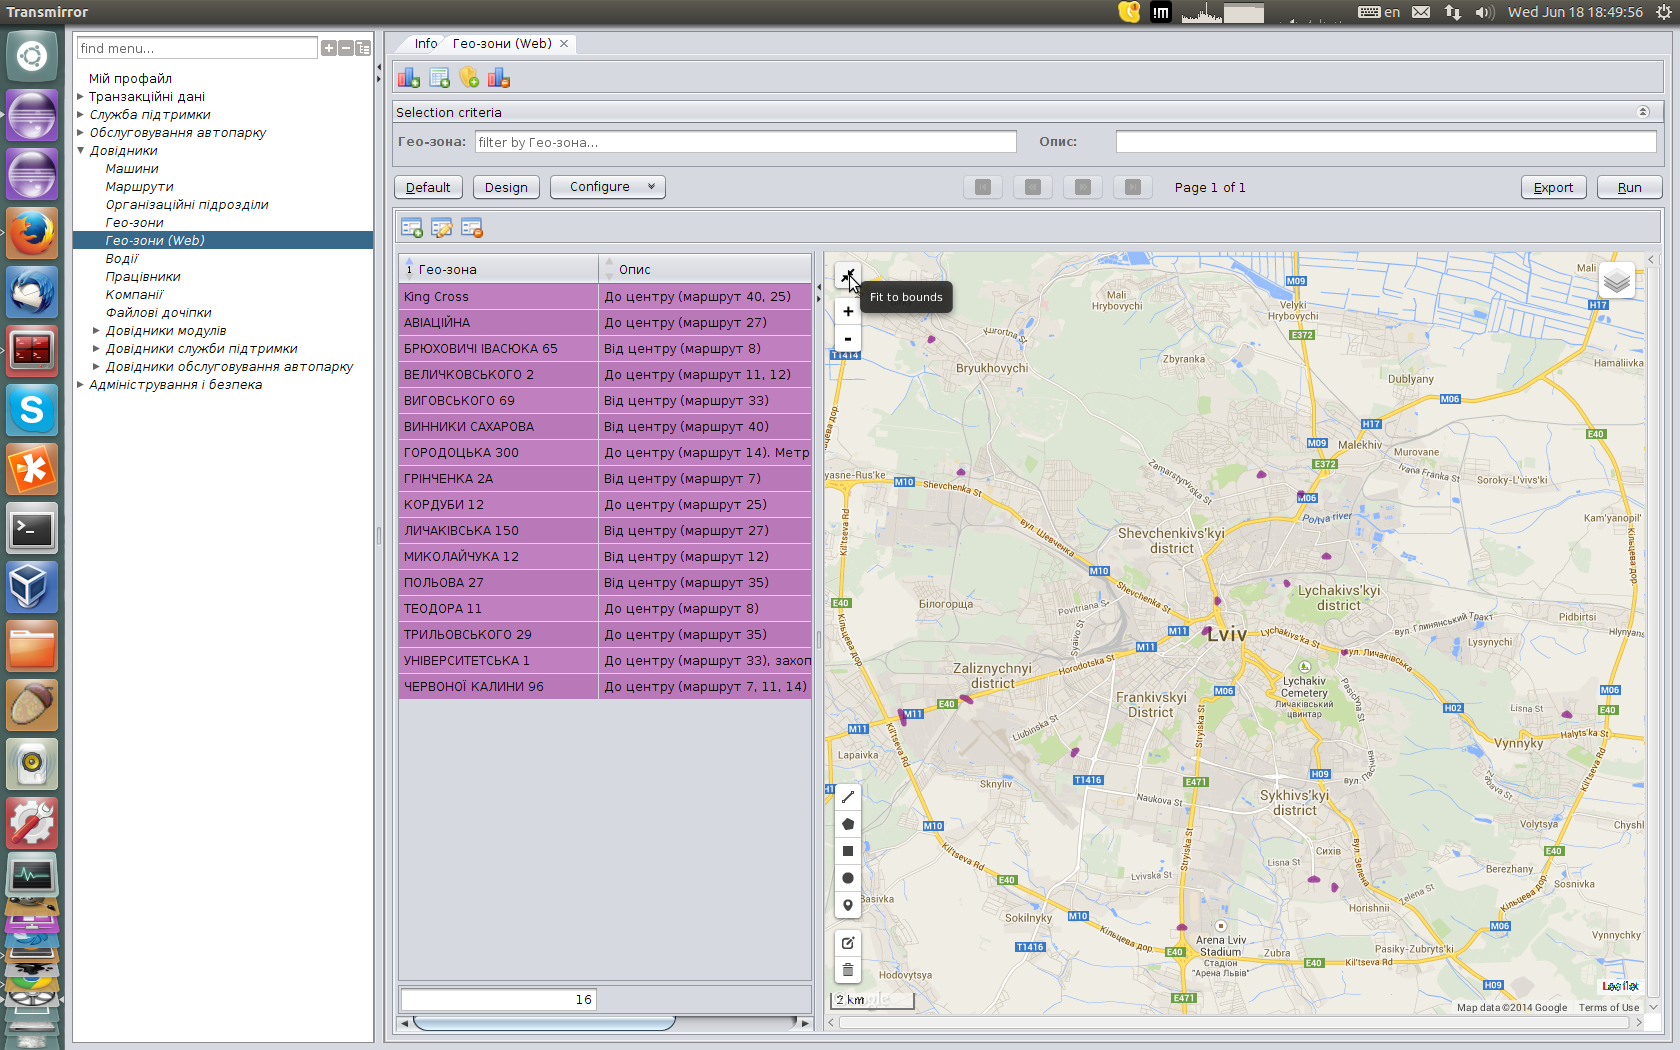
\includegraphics[width=\linewidth]{chapters/01-geozones/images/01-all-geo-zones-using-fit-to-bounds-button.png}
\caption{Positioning of all Geo-zones using ``Fit To Bounds'' button}\label{fig:01}
\end{figure}

\newpage
The necessary details can be viewed using zooming feature. Zooming can be done traditionally with mouse wheel button and a pair of zooming buttons ``+'' and ``-''. Also the user can press SHIFT button in conjuction with mouse selection and it works as a convenient zooming method (figure~\ref{fig:02}). It is very useful when some specific rectagular geo-area is interested in. 

\begin{figure}[H]
\centering
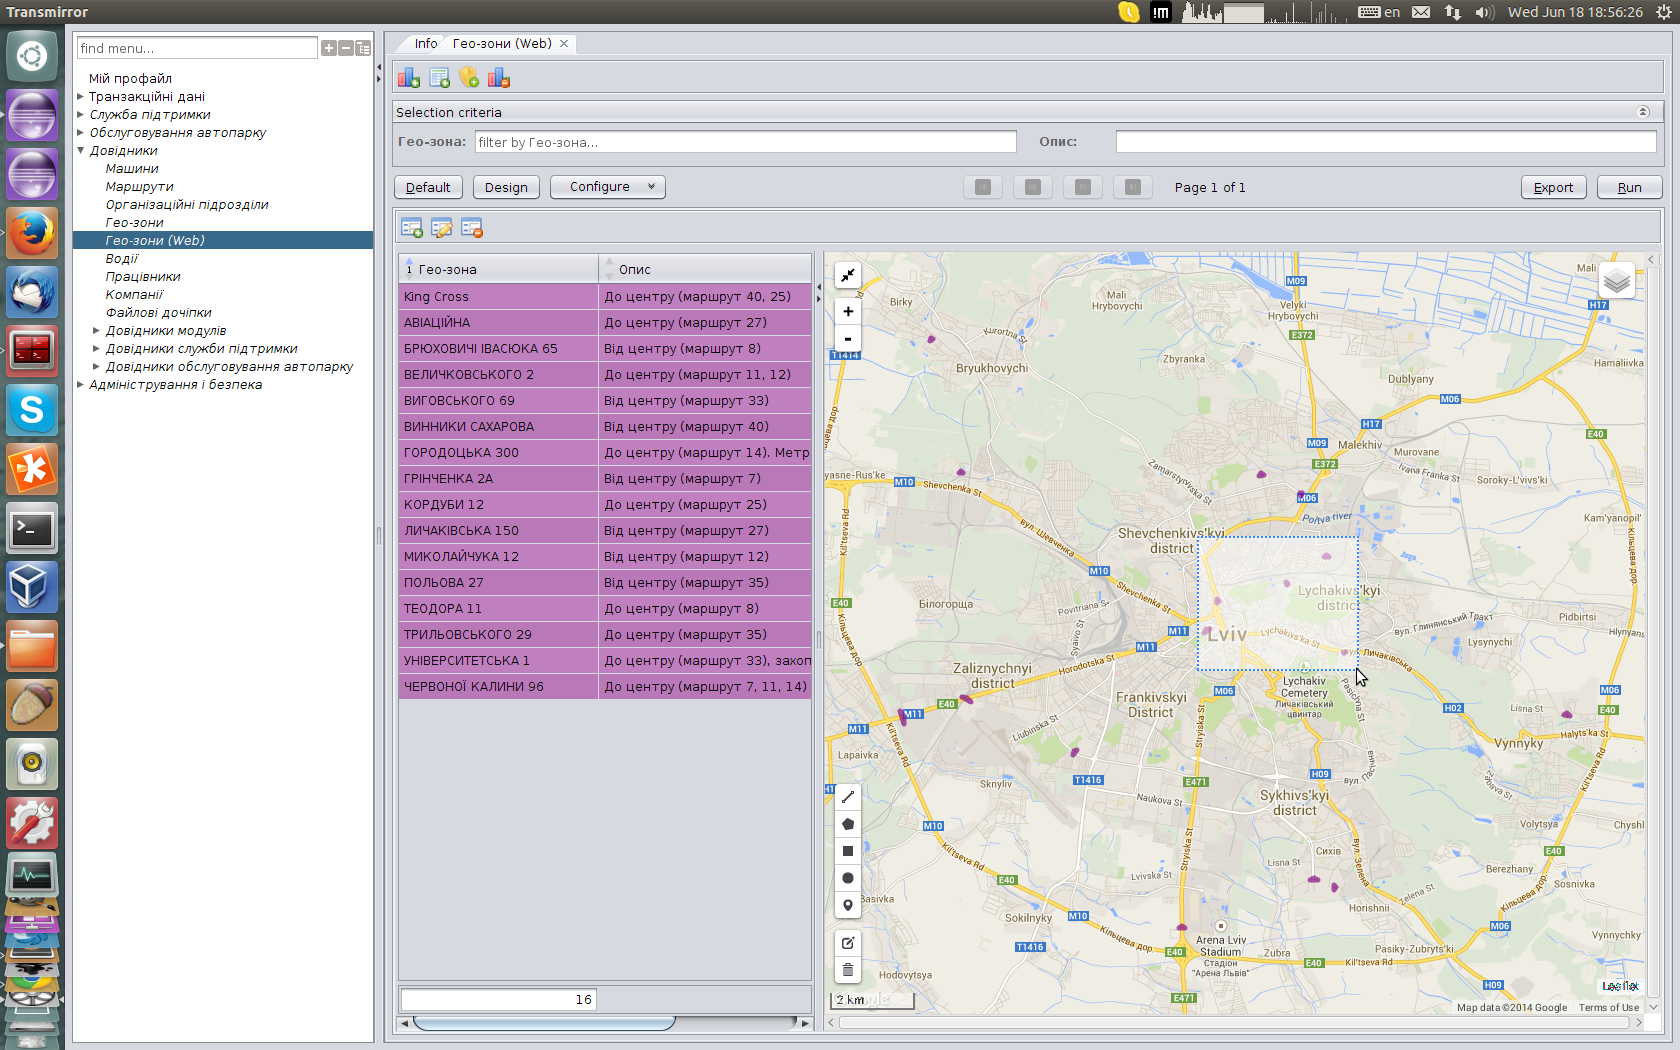
\includegraphics[width=\linewidth]{chapters/01-geozones/images/02-part-of-geo-zones-using-shift+selection-zoom.png}
\caption{Zooming with SHIFT-selection: showing a part of Geo-zones}\label{fig:02}
\end{figure}

\newpage
The result of zooming shows that example Geo-zones has been represented as triangles (figure~\ref{fig:03}). But actually, directed vector-like Geo-zones have been used for Transmirror project. The triangular shape has been only chosen to express the direction in which the vehicle should move through the Geo-zone to make an intersection. It resolves a common problem with GIS software -- intersection of Geo-zones by moving in opposite ways on the same road section. No distiction can be provided if Geo-zone has no ``direction'' concept assigned.

The shapes are not limited only by triangles -- complex polygons or circles can be used as well (see later figure~\ref{fig:07}). This is handy when a precise geozone shape of some specific nature is needed (for e.g. parking area or field).

The another convenient way to zoom to some concrete node is to just click on it (figure~\ref{fig:03}).

\begin{figure}[H]
\centering
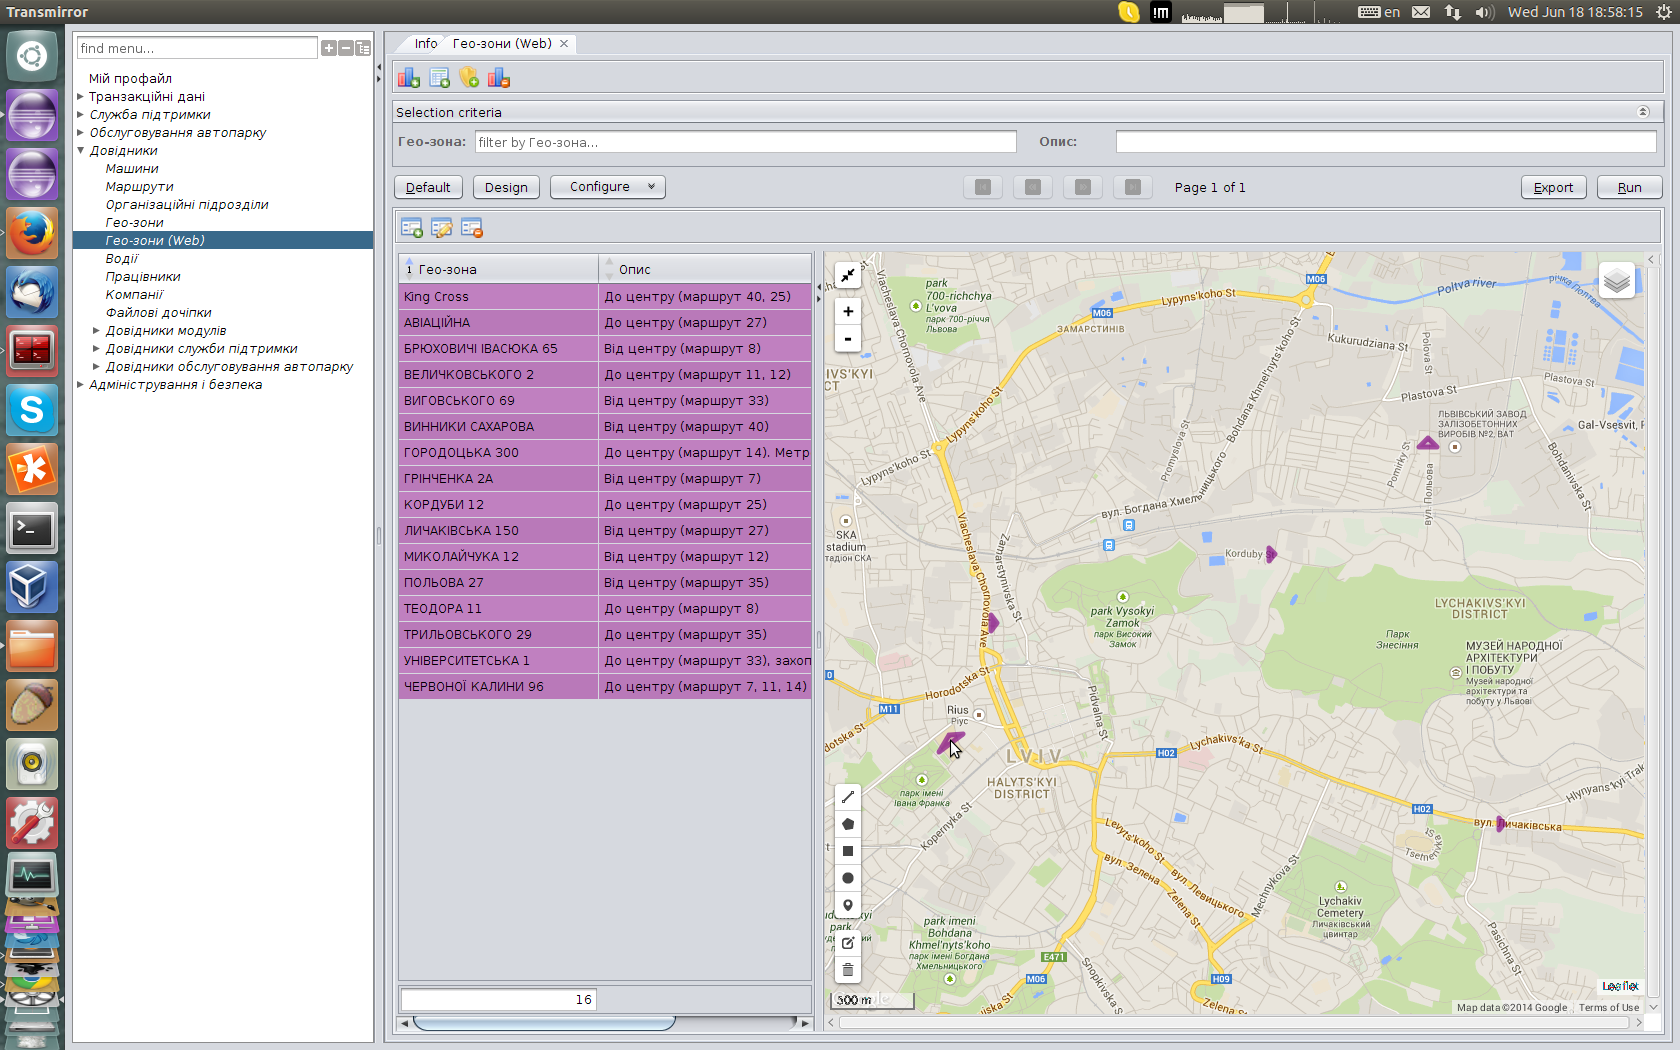
\includegraphics[width=\linewidth]{chapters/01-geozones/images/03-part-of-geo-zones-with-particular-item-selection-by-clicking.png}
\caption{Part of Geo-zones with particular item selection by clicking}\label{fig:03}
\end{figure}

\newpage
Clicking on triangle will fit it to the bounds of the map and will show the detailed popup information (figure~\ref{fig:04}). The table also will synchronise with the selected item (appropriate table row will also be selected). At this stage the table component is the regular Entity Grid Inspector that is used in all TG client applications. The development of Web-enabled EGI is on upcoming schedule.

\begin{figure}[H]
\centering
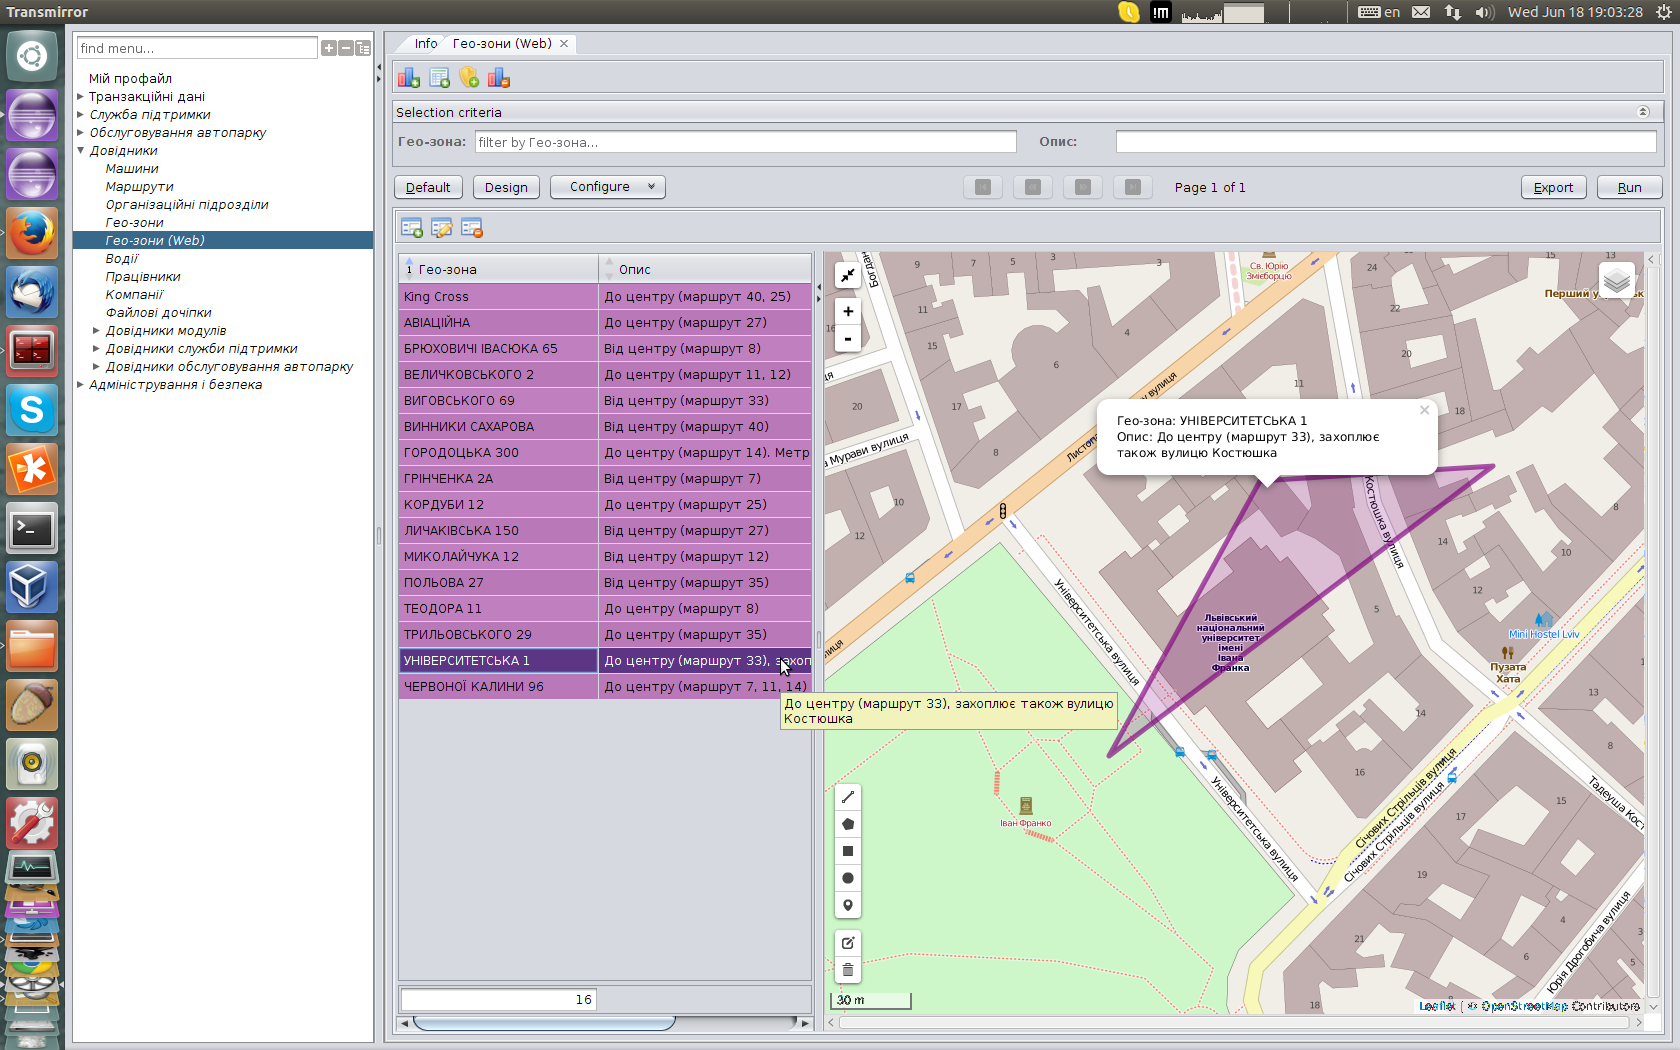
\includegraphics[width=\linewidth]{chapters/01-geozones/images/04-selected-geo-zone-and-synchronised-with-grid.png}
\caption{The Geo-zone has been selected and synchronised with Entity Grid Inspector}\label{fig:04}
\end{figure}

\newpage
Editing of Geo-zones is also supported by dragging polygon corners (figure~\ref{fig:05}). Appropriate shape can be formed with arbitrary number of corners -- the ``greyed-out'' corners (in the middle of the line segments) should be used to extend number of corners. The changes can be simply discarded if needed using ``Cancel" button or saved with ''Save" button.

\begin{figure}[H]
\centering
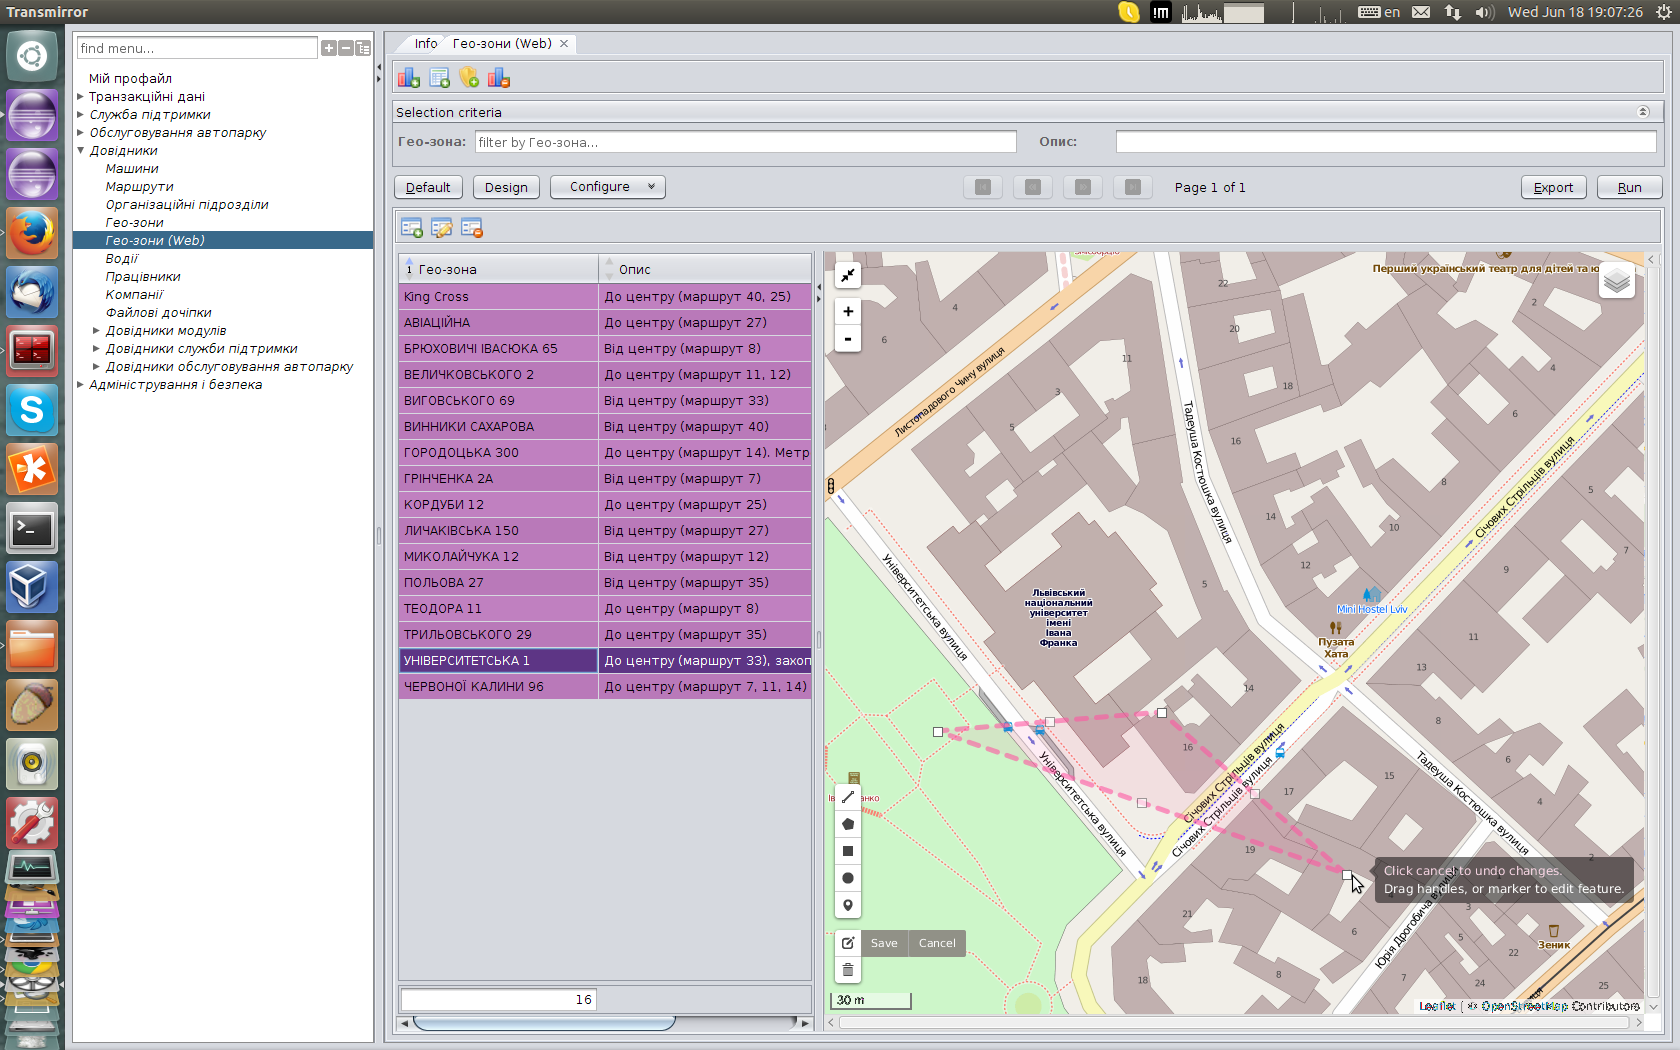
\includegraphics[width=\linewidth]{chapters/01-geozones/images/05-editing-geo-zone-using-graphical-interface.png}
\caption{Geo-zone editing using graphical interface}\label{fig:05}
\end{figure}

\newpage
The result of editing is a regular shape (figure~\ref{fig:06}) that can be used exactly the same as the previous version.

\begin{figure}[H]
\centering
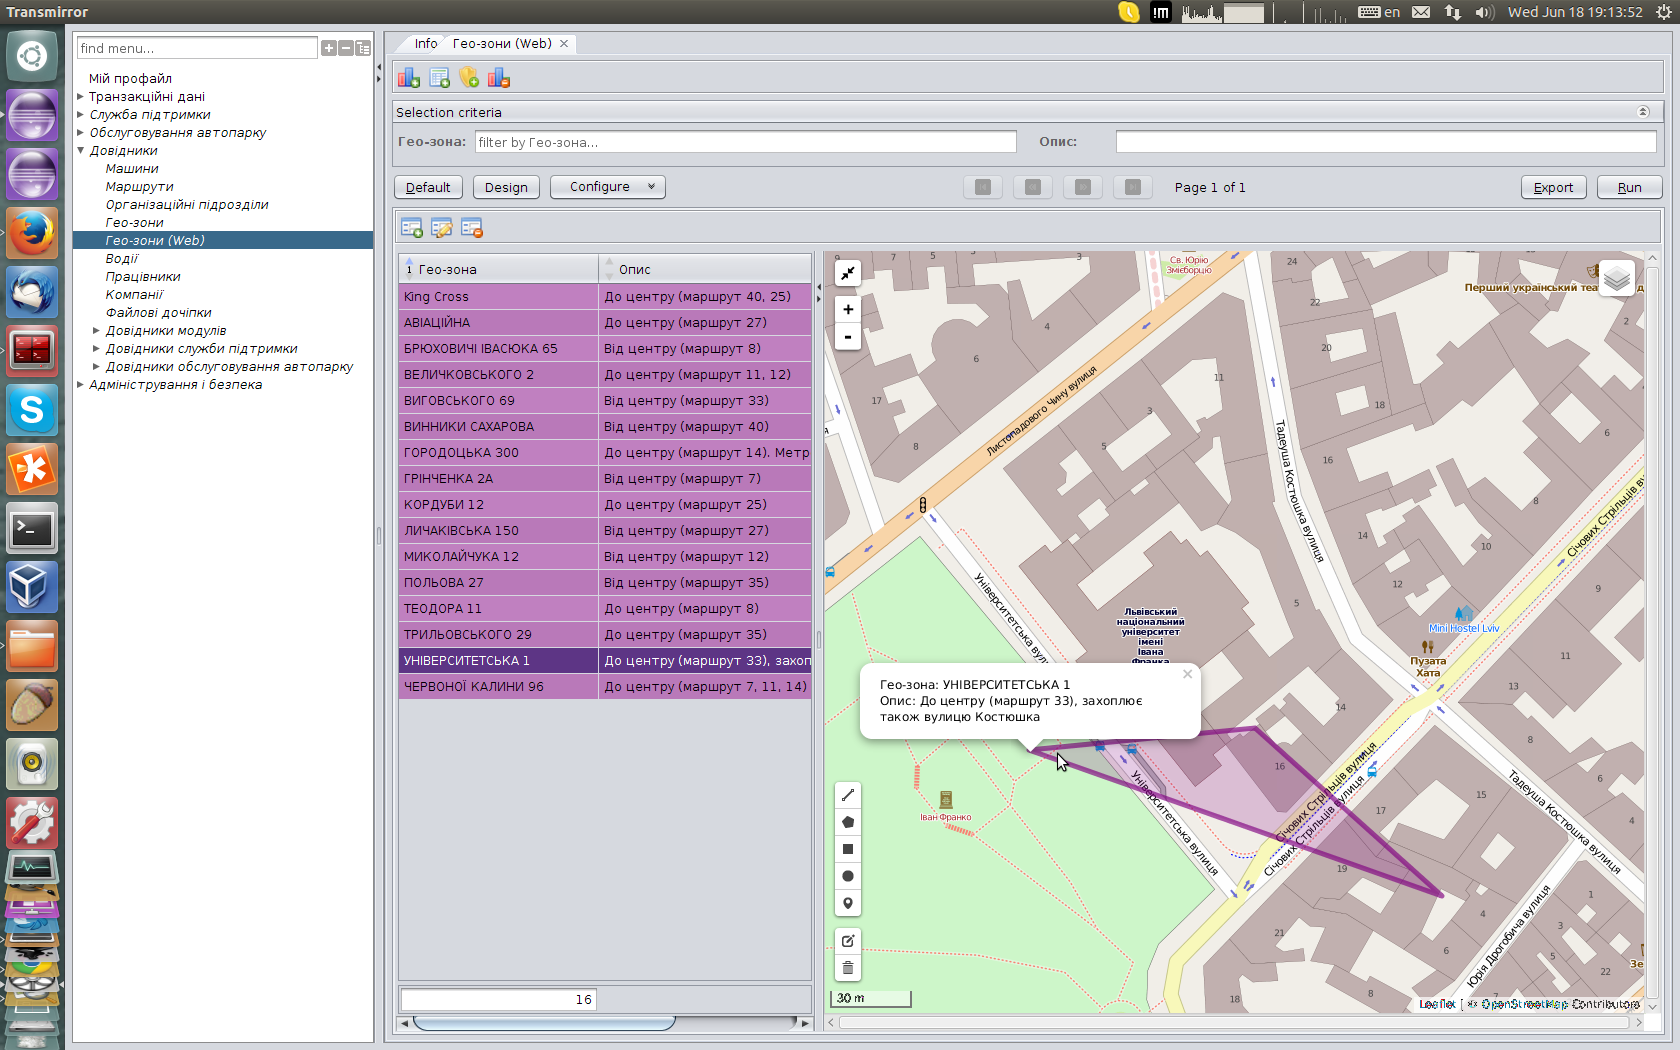
\includegraphics[width=\linewidth]{chapters/01-geozones/images/06-edited-geo-zone.png}
\caption{Edited Geo-zone}\label{fig:06}
\end{figure}

\newpage
As has been mentioned before, complex shapes can be used (figure~\ref{fig:07}). These include circles, rectangles or polygons. The area amount is also calculated during polygon editing.

\begin{figure}[H]
\centering
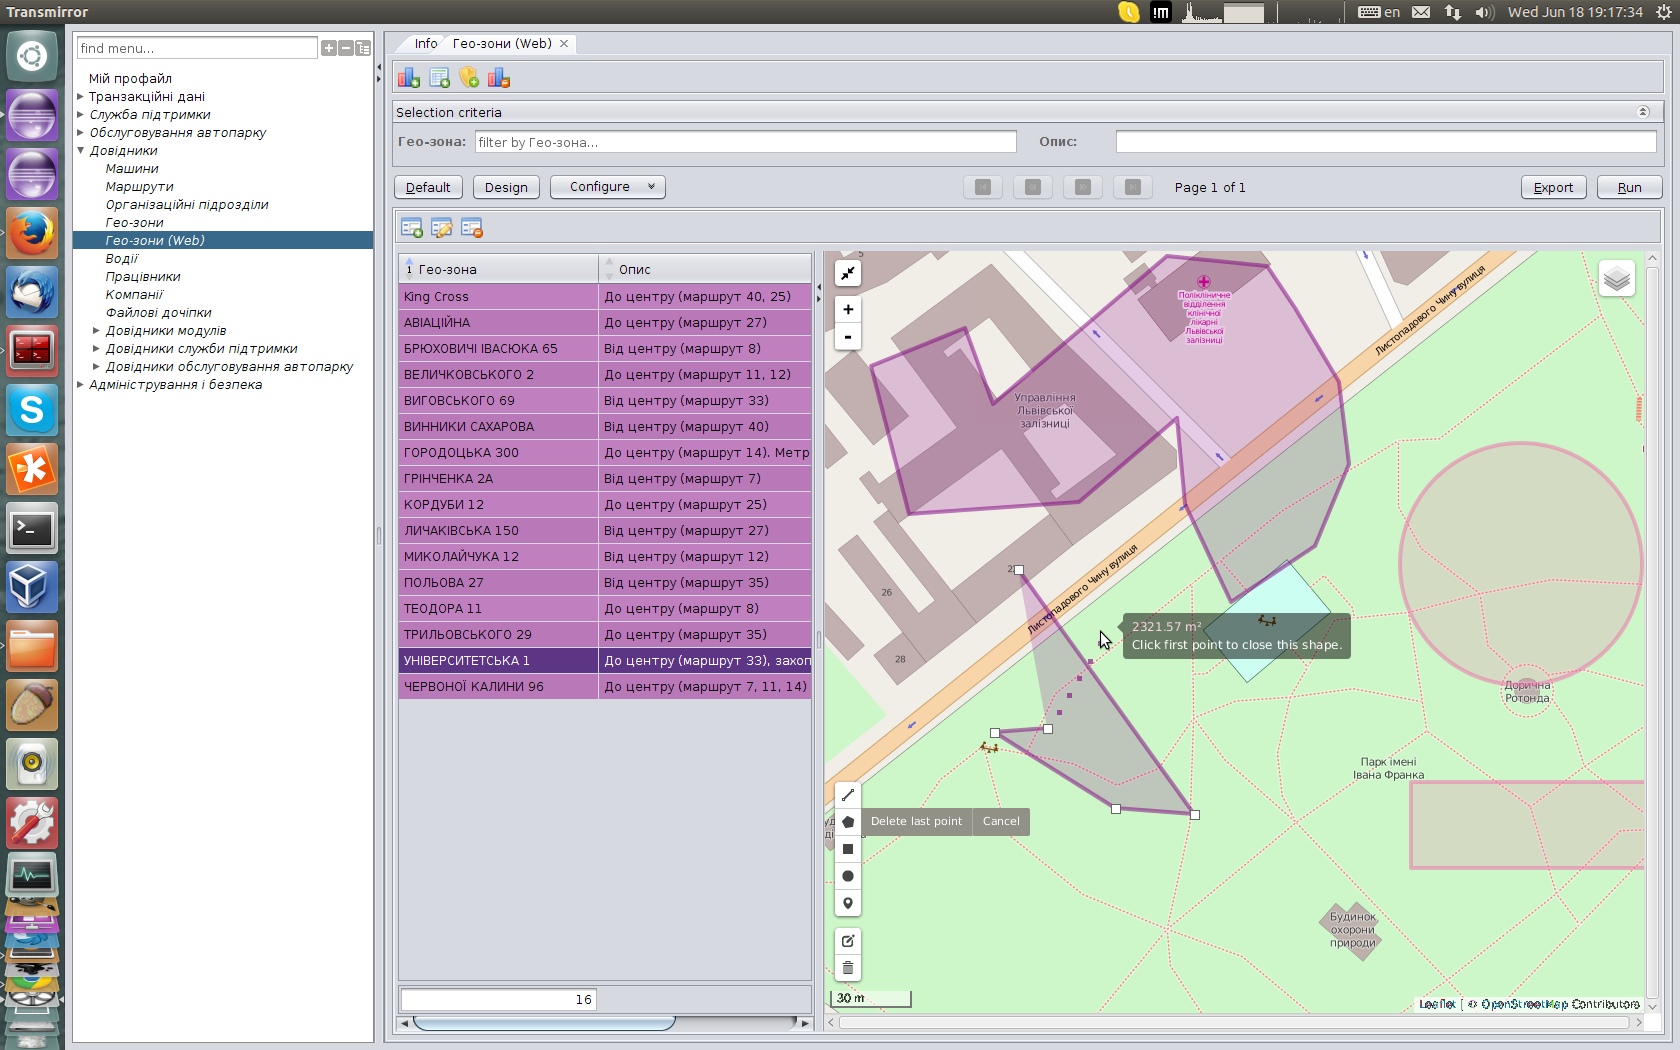
\includegraphics[width=\linewidth]{chapters/01-geozones/images/07-creating-new-complex-geo-zones.png}
\caption{Creating new complex Geo-zones}\label{fig:07}
\end{figure}

\newpage
Validation for the shape is necessary to make possible only meaninful Geo-zones (the edges should not cross). This is also done during editing as the area amount calculation (figure~\ref{fig:08}).

\begin{figure}[H]
\centering
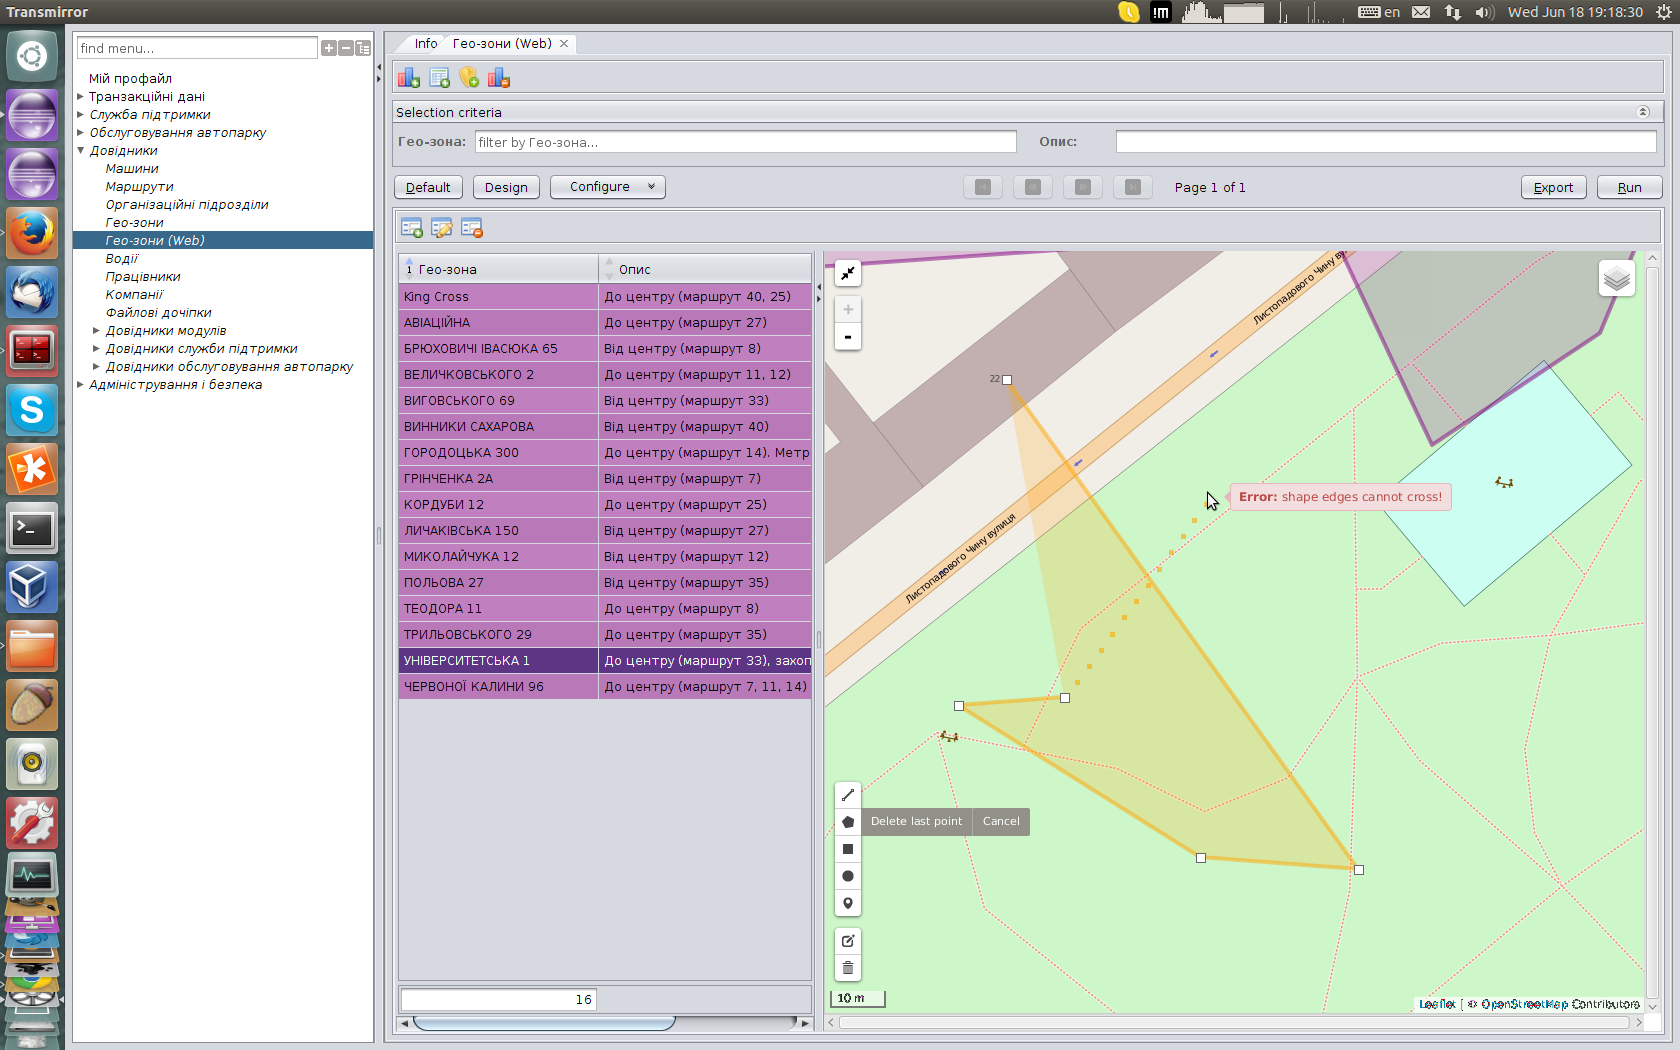
\includegraphics[width=\linewidth]{chapters/01-geozones/images/08-validation-for-complex-polygonial-geozone.png}
\caption{Validation for complex polygonial Geo-zone}\label{fig:08}
\end{figure}

\newpage
Map service changing is easily done by clicking on right top button. Basically tile services are not limited only by OpenStreetMap, Google, Yandex and Landscape, but at this stage only those are supported (figure~\ref{fig:09}). Please also note that several types of tiles for the same provider is available (for e.g. Sattelite, Roadmap or Terrain).

\begin{figure}[H]
\centering
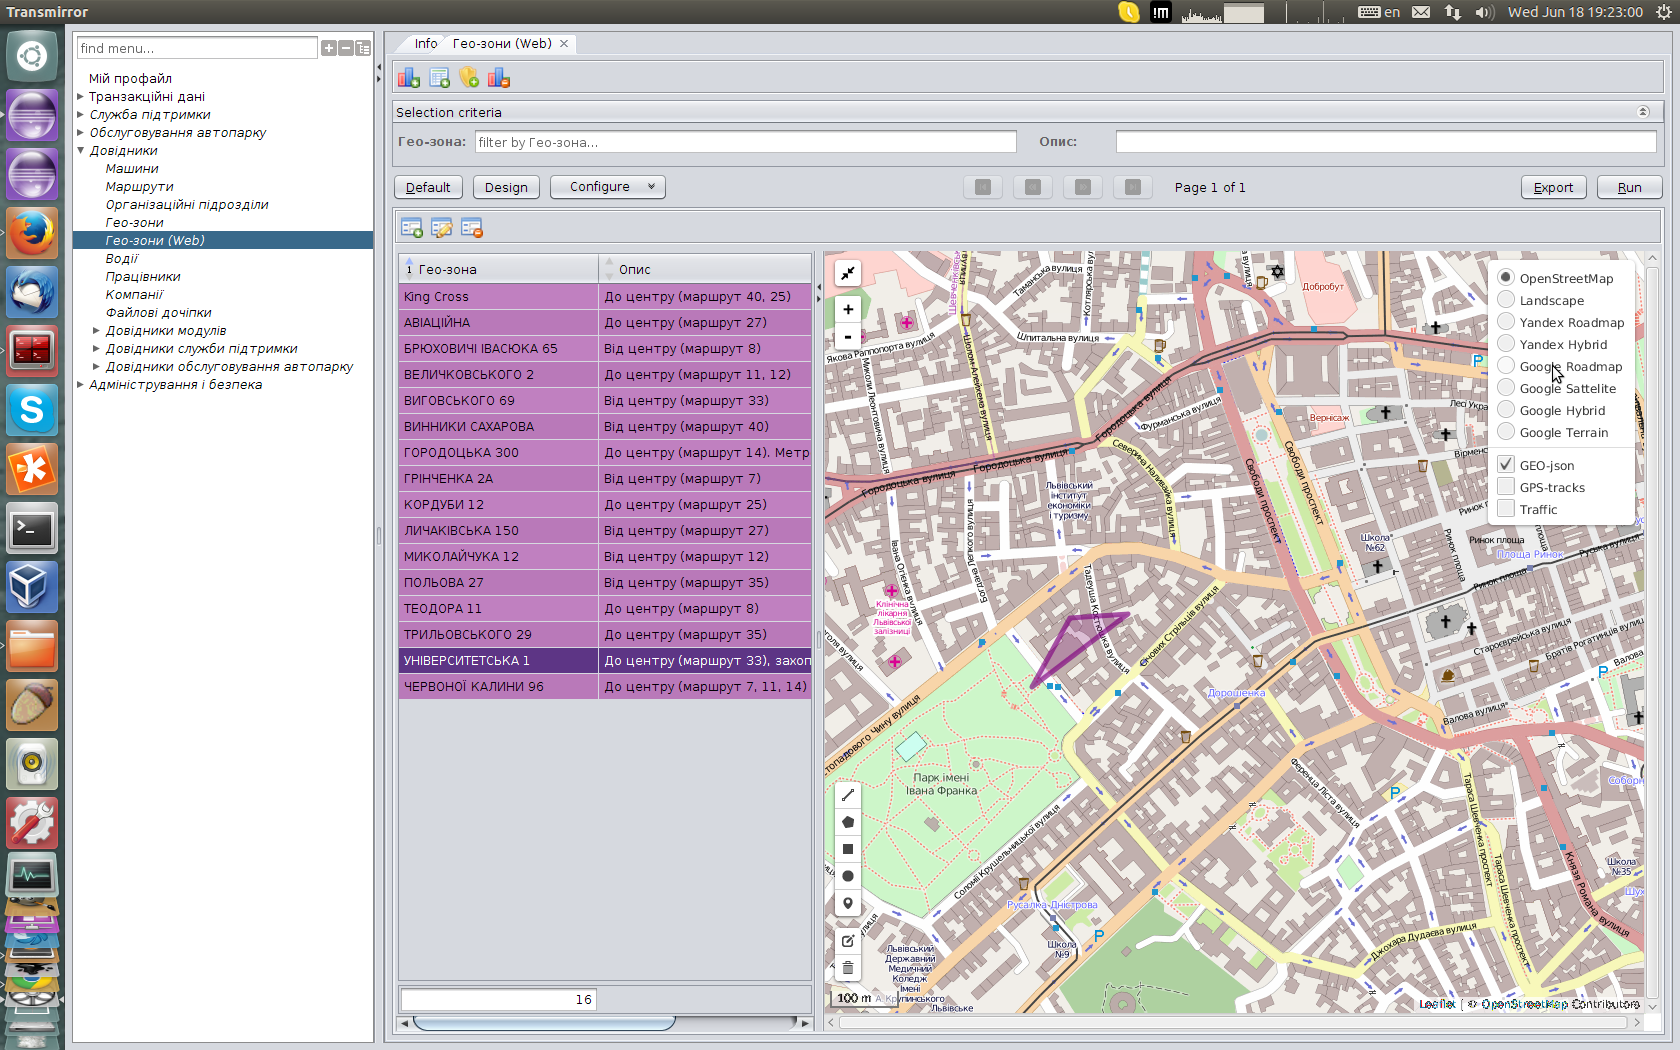
\includegraphics[width=\linewidth]{chapters/01-geozones/images/09-changing-map-tiling-service.png}
\caption{Changing map tiling service}\label{fig:09}
\end{figure}

\newpage
The result of map changing to Google Roadmap from OpenStreetMap.

\begin{figure}[H]
\centering
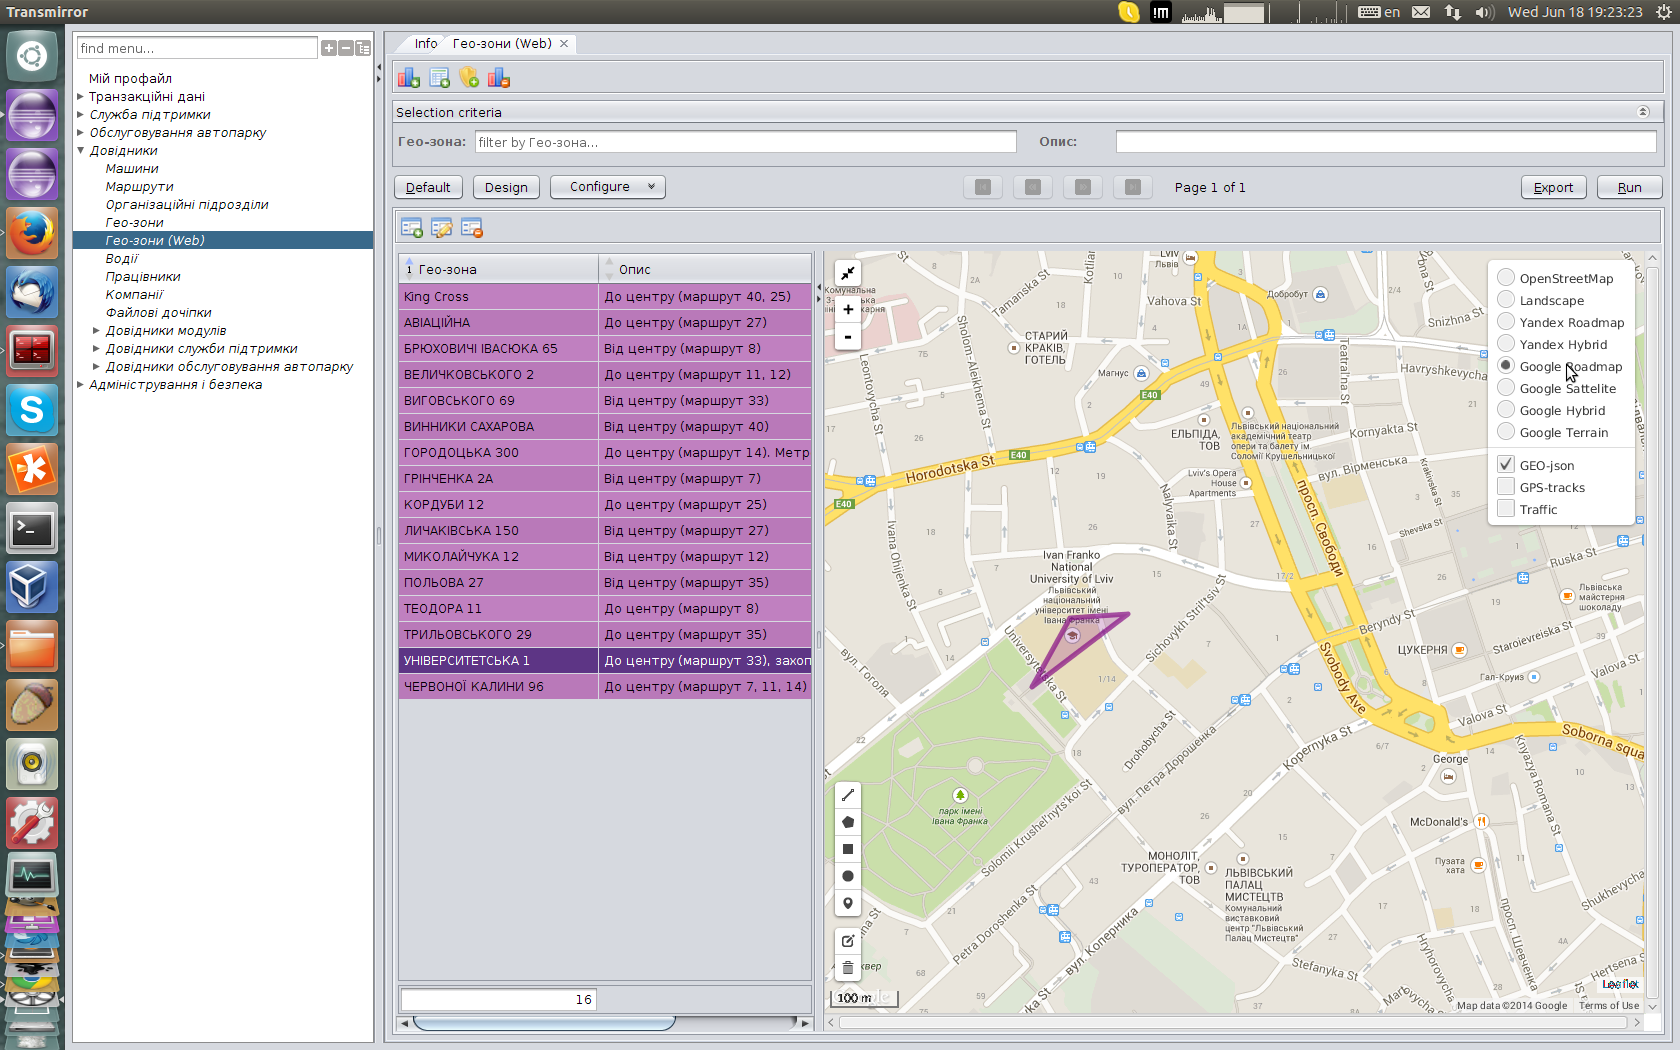
\includegraphics[width=\linewidth]{chapters/01-geozones/images/10-changed-map-tiling-service.png}
\caption{Changed map tiling service to Google Roadmap}\label{fig:10}
\end{figure}
  \section{GPS-tracks}

GPS-track is a common visual representation for machine path for some period of time. It can be used for detailed analysis of where and when the machine was located, what was the speed at concrete moment, where the stoppage has been occured etc.

This detailing analysis is useful when other more specific reports can not bring the necessary analysis granularity. For example, we need to determine the vehicle that travelled the most yesterday. In this case we use some aggregation report, possibly in tabular format, and sort the number of travelled kilometers descending. But why, where and exactly when the vehicle has been performed its route -- it can be analysed using GPS-tracks feature.

In figure~\ref{fig:11} the machine track for concrete period is shown. Whole track is divided on several regions which are commonly called ``clusters''. There are two types of clusters: 1) cluster with red marker which contain stoppages 2) cluster with blue ``directed'' marker with approximate direction of movement. The region is shown when the user hovers the cluster (figure~\ref{fig:11}). Cluster zooming can be done using single click action. 

\begin{figure}[H]
\centering
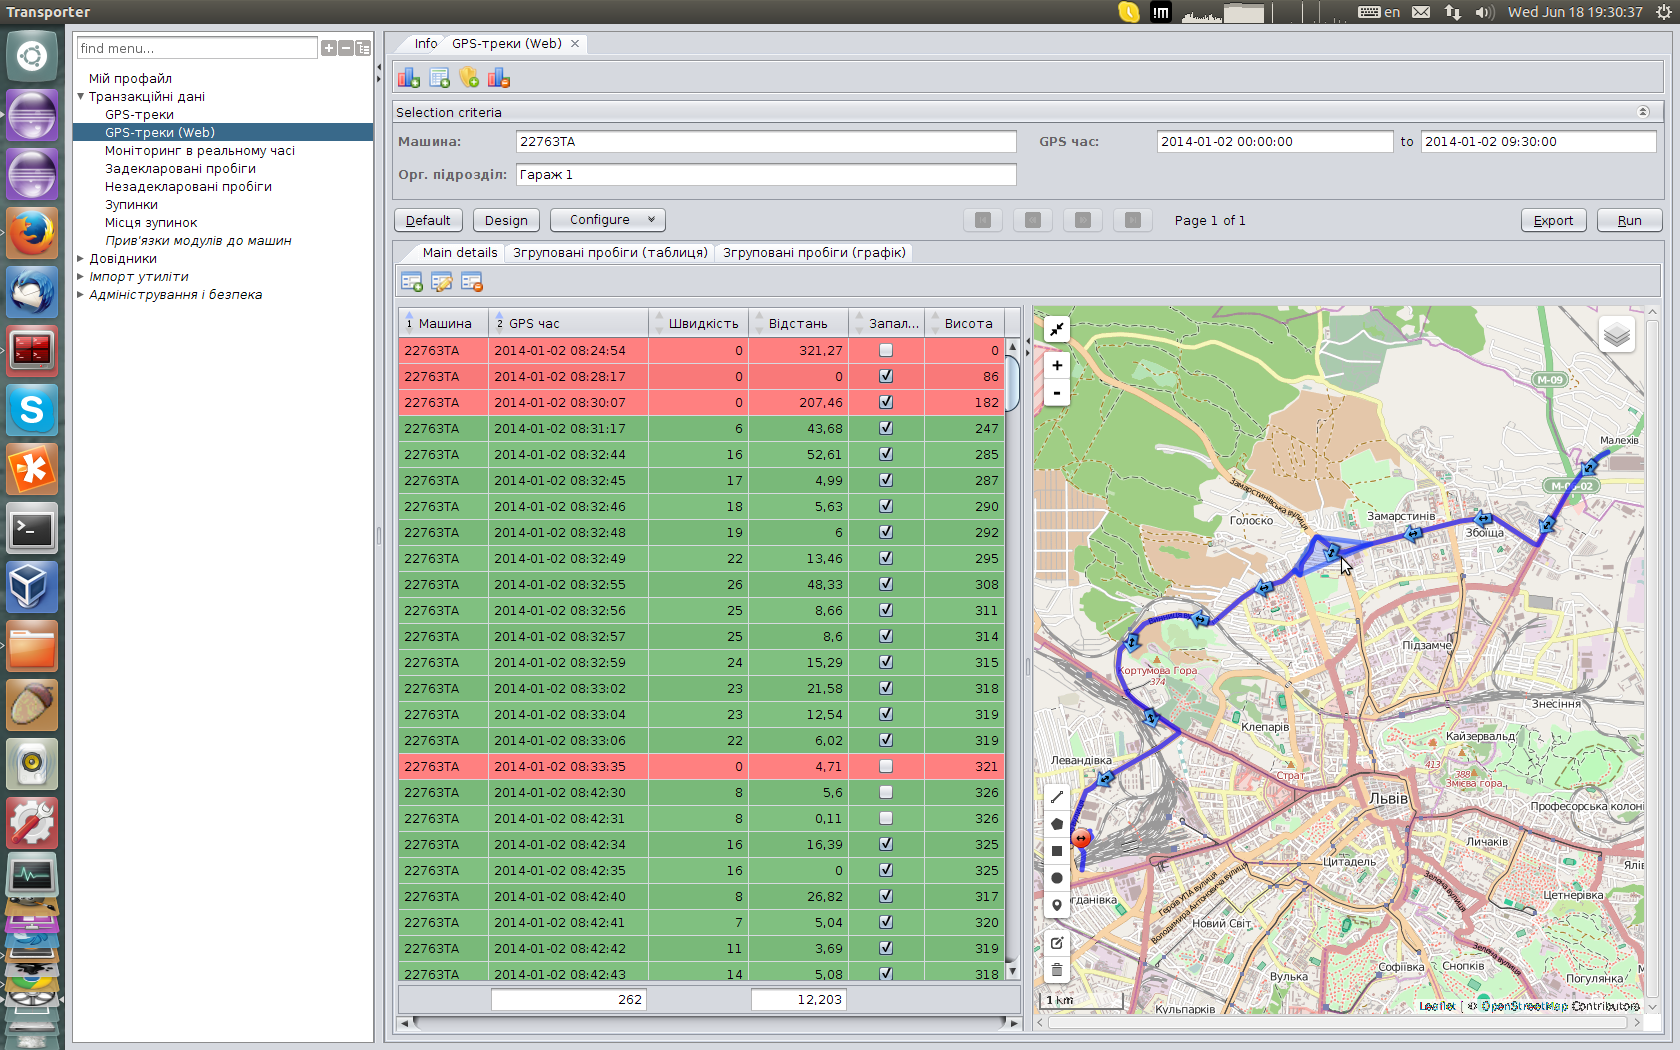
\includegraphics[width=\linewidth]{chapters/02-gpstracks/images/11-clusterised-gps-track-view-with-hovered-cluster.png}
\caption{Clusterised GPS-track view with hovered cluster}\label{fig:11}
\end{figure}

\newpage
Zooming to concrete region using clicking on a cluster is very handy and conveniently. Typical scenario of usage is to analyse which was the track in some particular place. The result of clicking is shown on figure~\ref{fig:12} -- the smaller part of track has been clusterised. The animation of nodes and map is used during zooming to better follow by zooming process.

\begin{figure}[H]
\centering
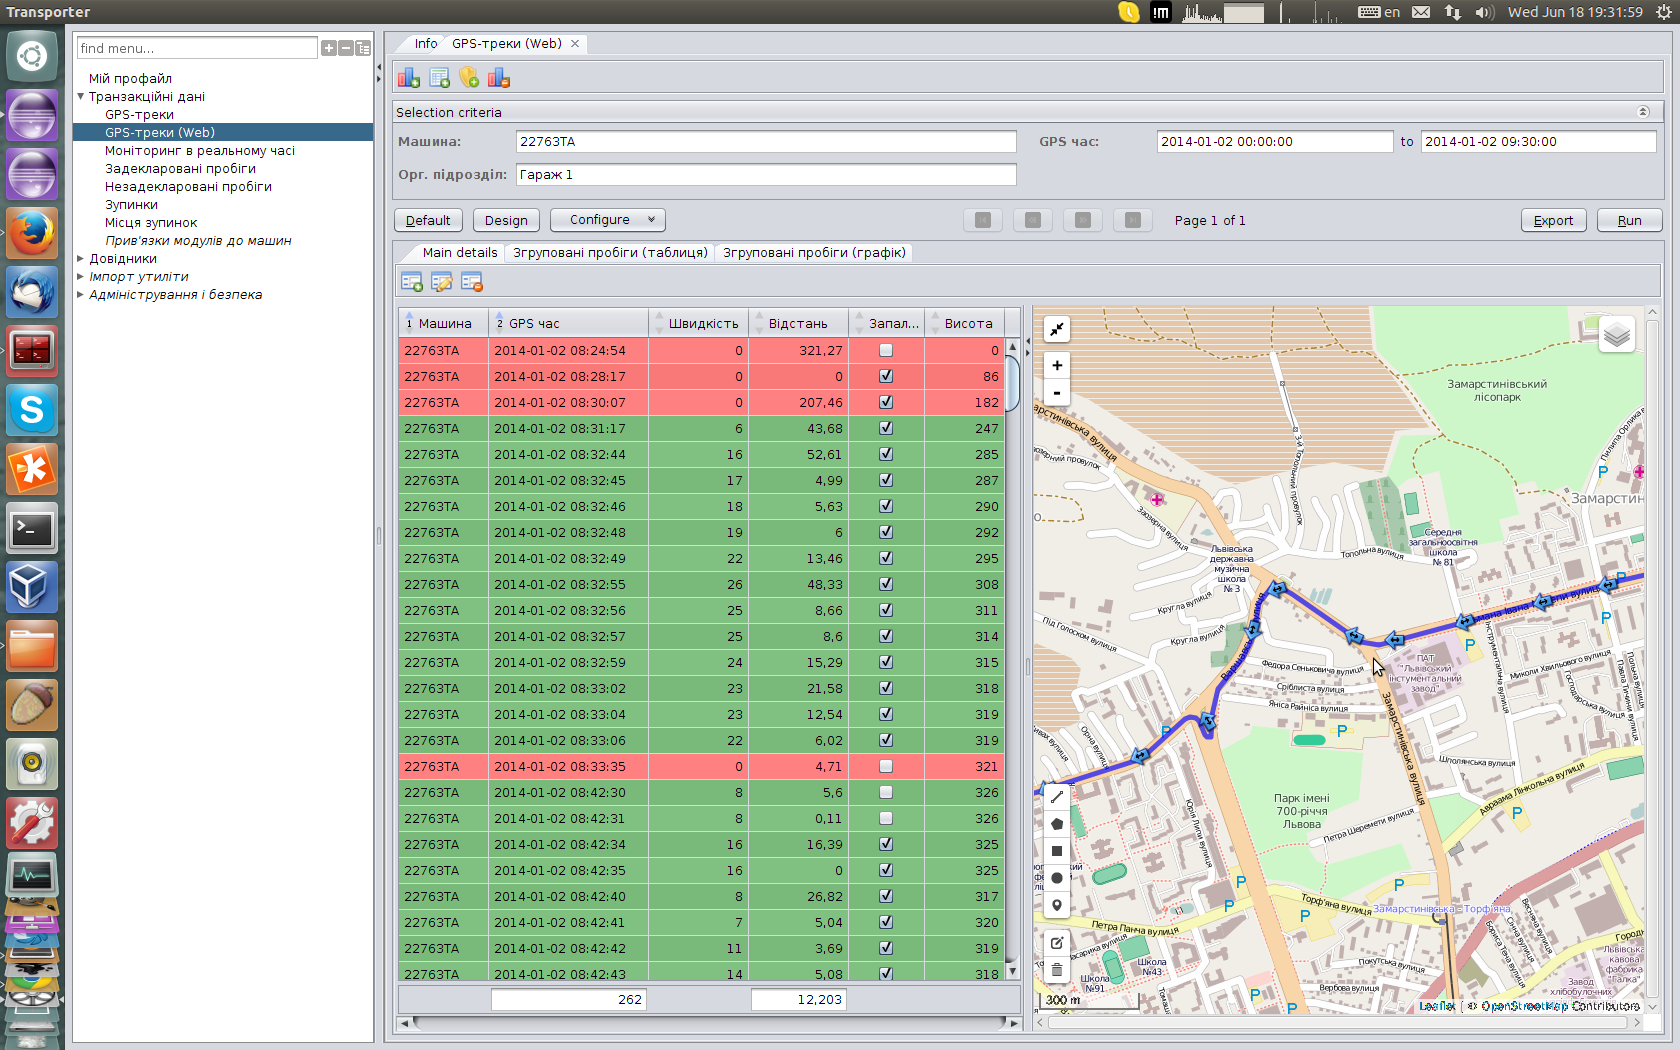
\includegraphics[width=\linewidth]{chapters/02-gpstracks/images/12-zooming-by-clicking-a-cluster.png}
\caption{Zoomed cluster region after the cluster has been clicked}\label{fig:12}
\end{figure}

\newpage
If the user clicks on some smaller cluster -- the detailed GPS-track is appeared with concrete GPS-messages (figure~\ref{fig:13}). The directions of the messages are precise enough to the level which GPS-module provides. 

\begin{figure}[H]
\centering
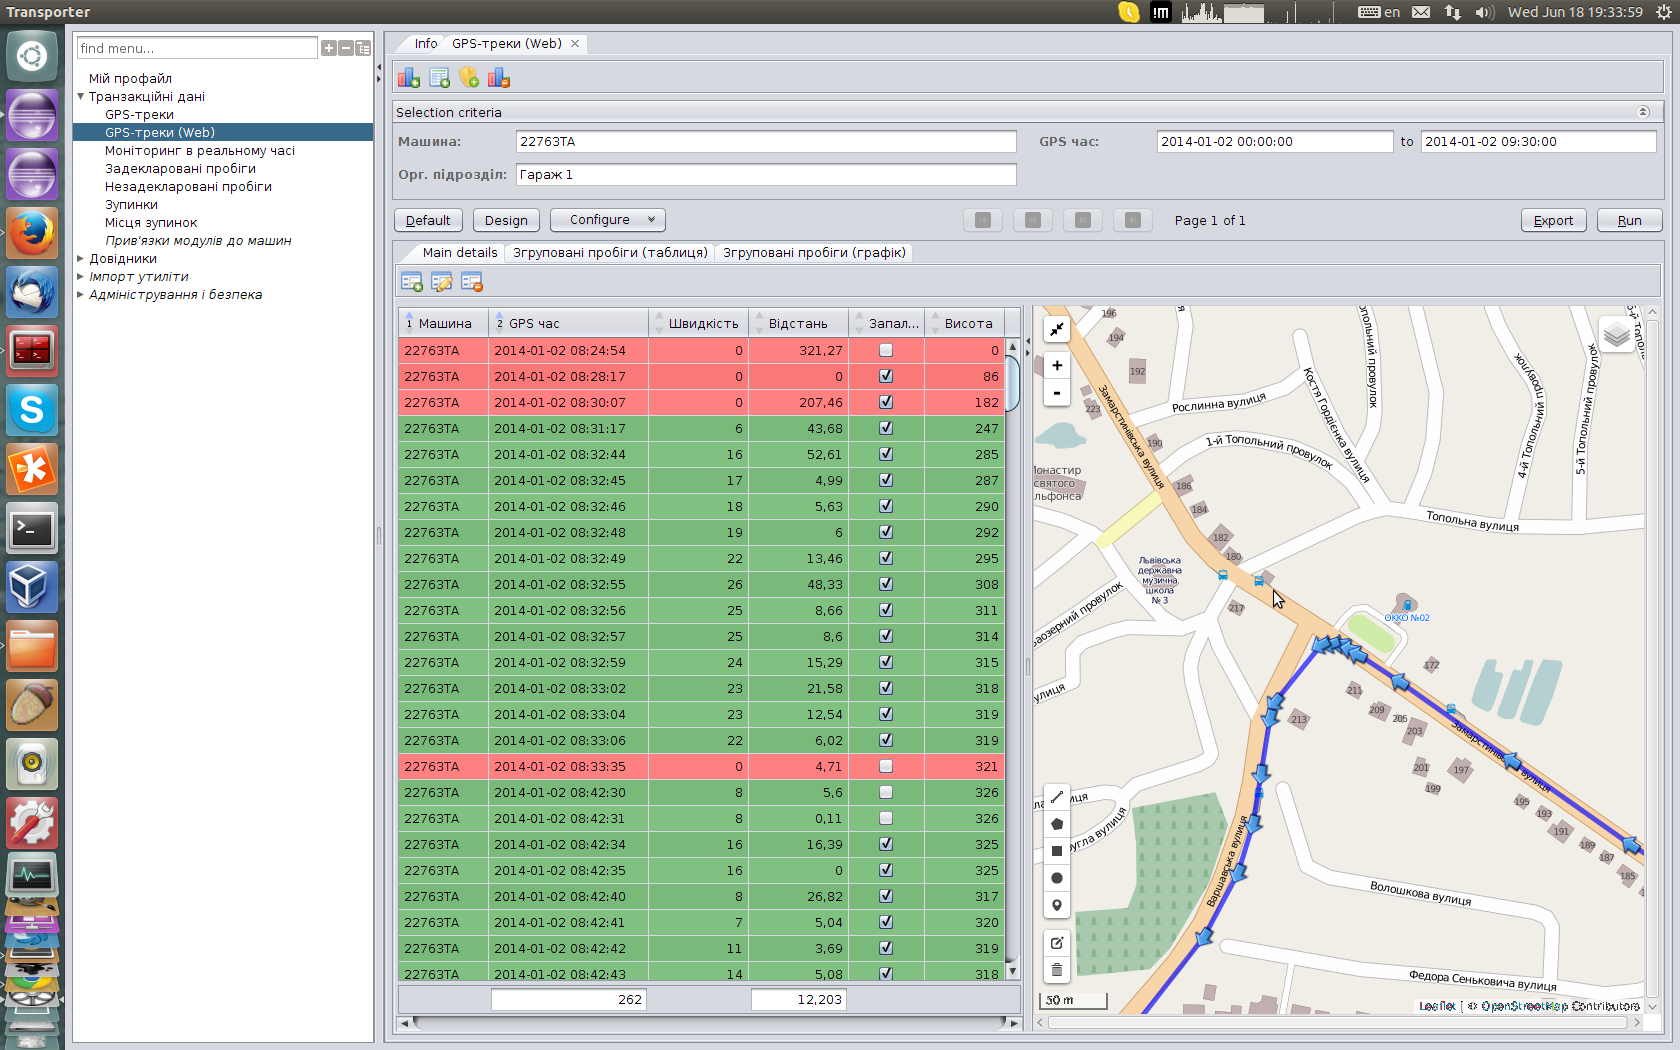
\includegraphics[width=\linewidth]{chapters/02-gpstracks/images/13-detailed-gps-track-view.png}
\caption{Detailed GPS-track view}\label{fig:13}
\end{figure}

\newpage
If the user clicks on red cluster -- the smaller part of track clusterises (figure~\ref{fig:14}). Small stoppage clusters are shown in this case which means that the vehicle made stoppages in all that places.

\begin{figure}[H]
\centering
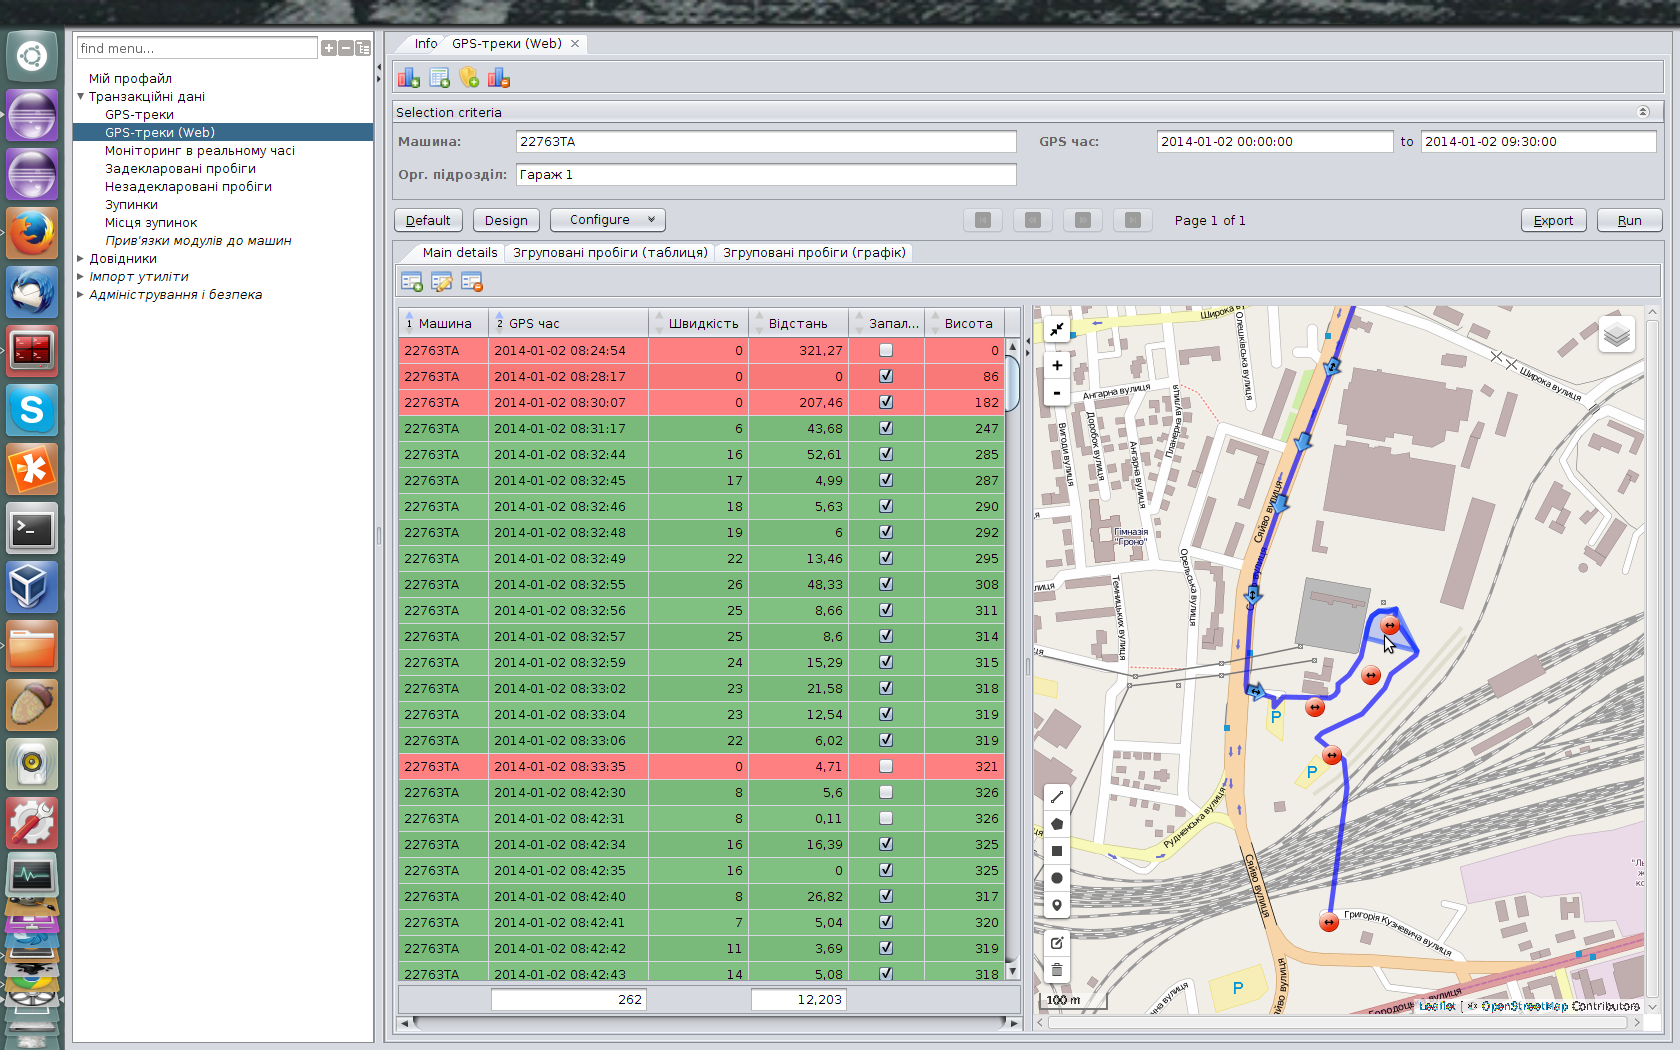
\includegraphics[width=\linewidth]{chapters/02-gpstracks/images/14-clusters-with-stoppage-messages-with-zero-speed.png}
\caption{Clusters with stoppage messages with zero speed}\label{fig:14}
\end{figure}

\newpage
If the user clicks on some smaller cluster -- the detailed GPS-track is appeared with concrete GPS-messages which include zero-speed messages (figure~\ref{fig:15}).

\begin{figure}[H]
\centering
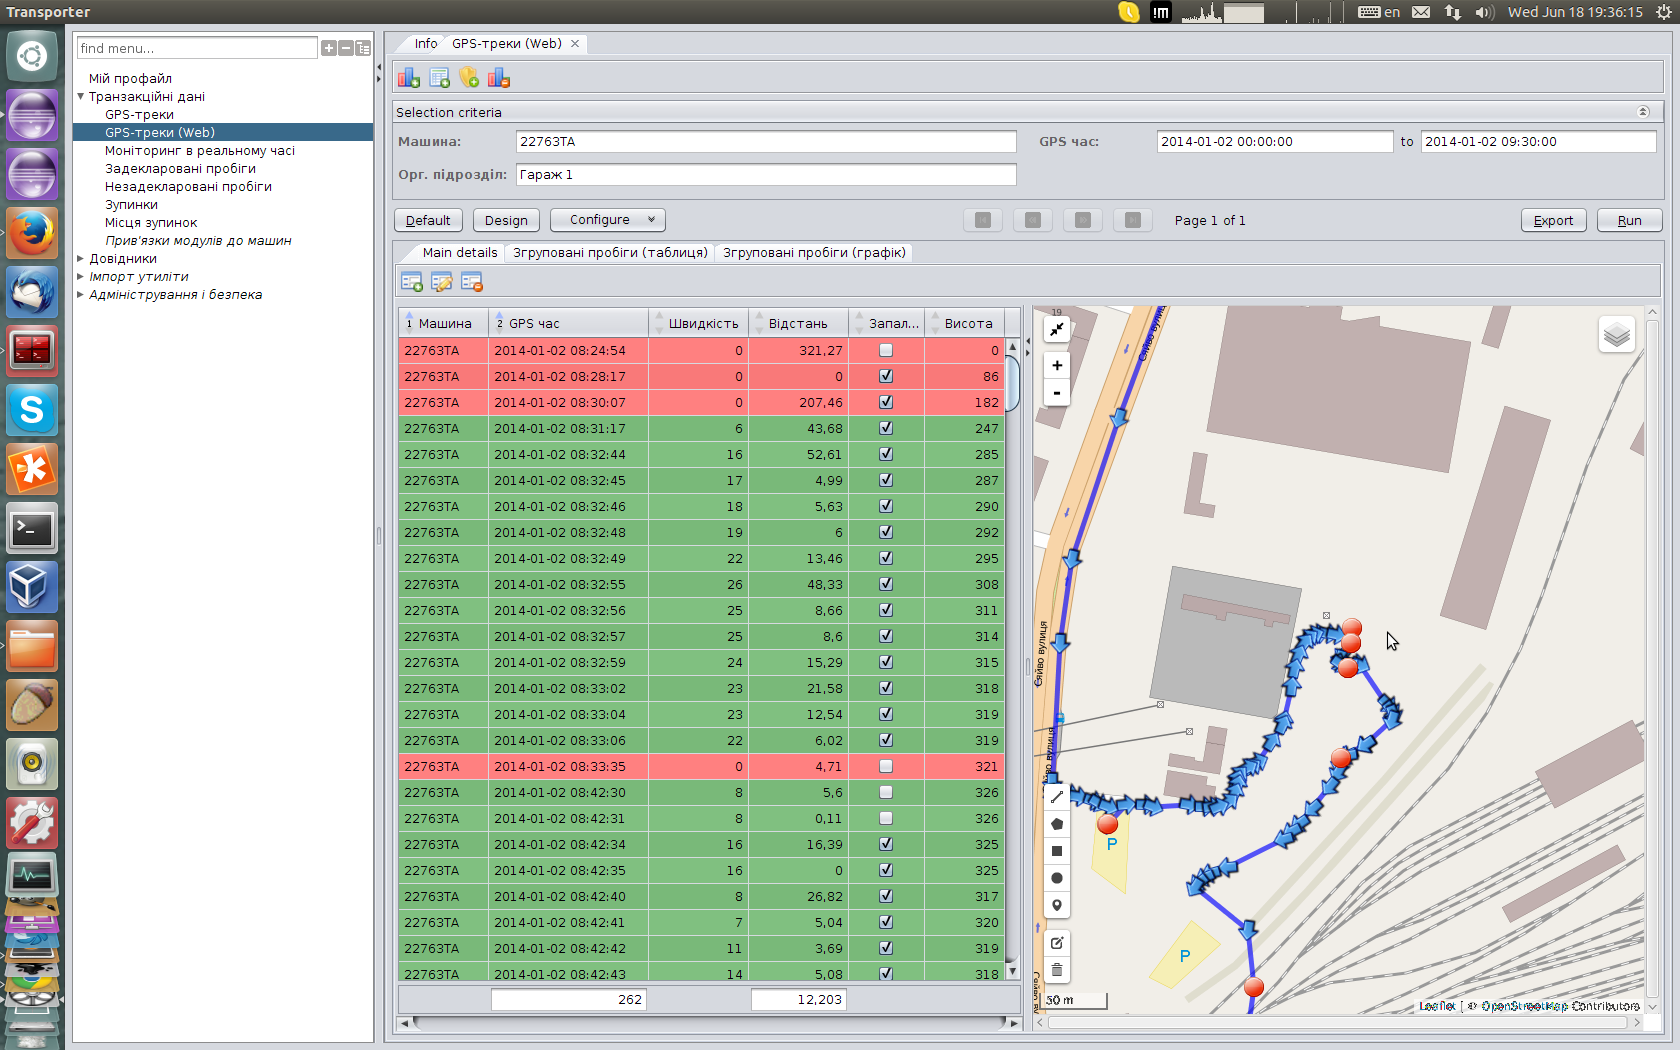
\includegraphics[width=\linewidth]{chapters/02-gpstracks/images/15-detailed-view-with-stoppages.png}
\caption{Detailed view with stoppages}\label{fig:15}
\end{figure}

\newpage
Concrete message details can be reviewed using message selection -- simple clicking action (figure~\ref{fig:16}). The popup shows and colouring of the message changes to green after selection. Please also note that appropriate grid row is also selected. 

If the user hovers the track messages they will appear to the top. Also the stoppage message is always on top to draw user's attention.

\begin{figure}[H]
\centering
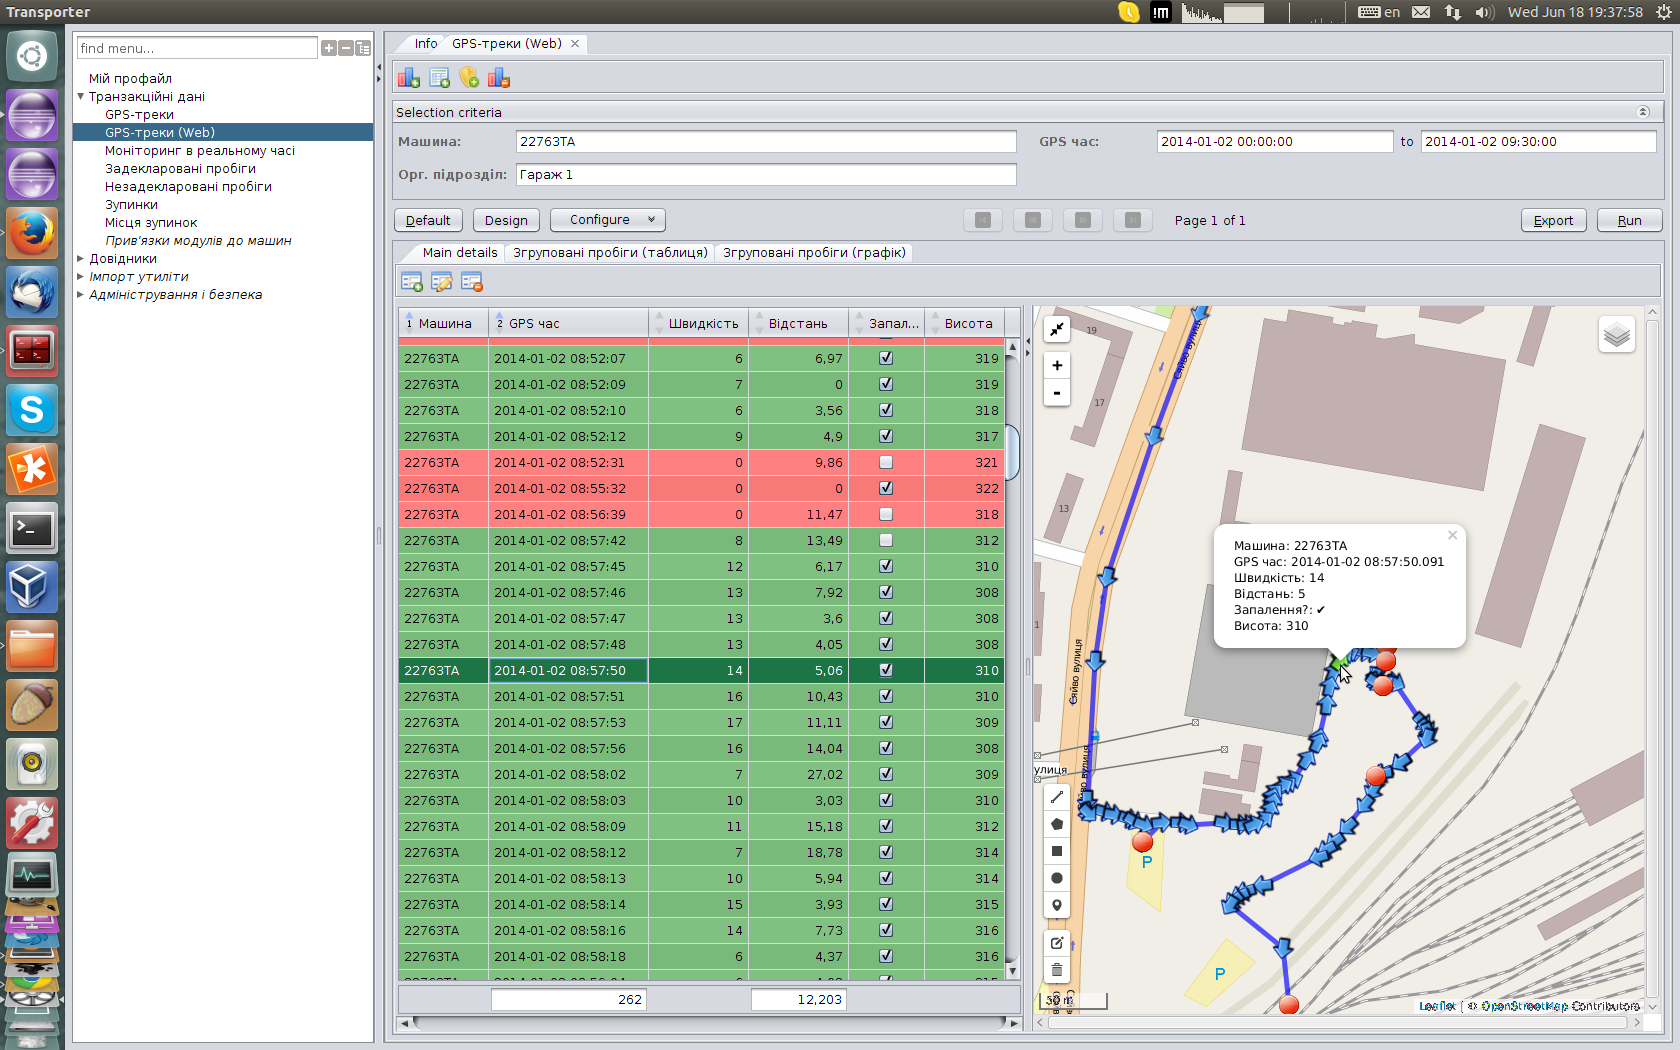
\includegraphics[width=\linewidth]{chapters/02-gpstracks/images/16-selected-message-with-popup.png}
\caption{Selected message with popup}\label{fig:16}
\end{figure}

\newpage
Selected stoppage message is shown on figure~\ref{fig:17}.

\begin{figure}[H]
\centering
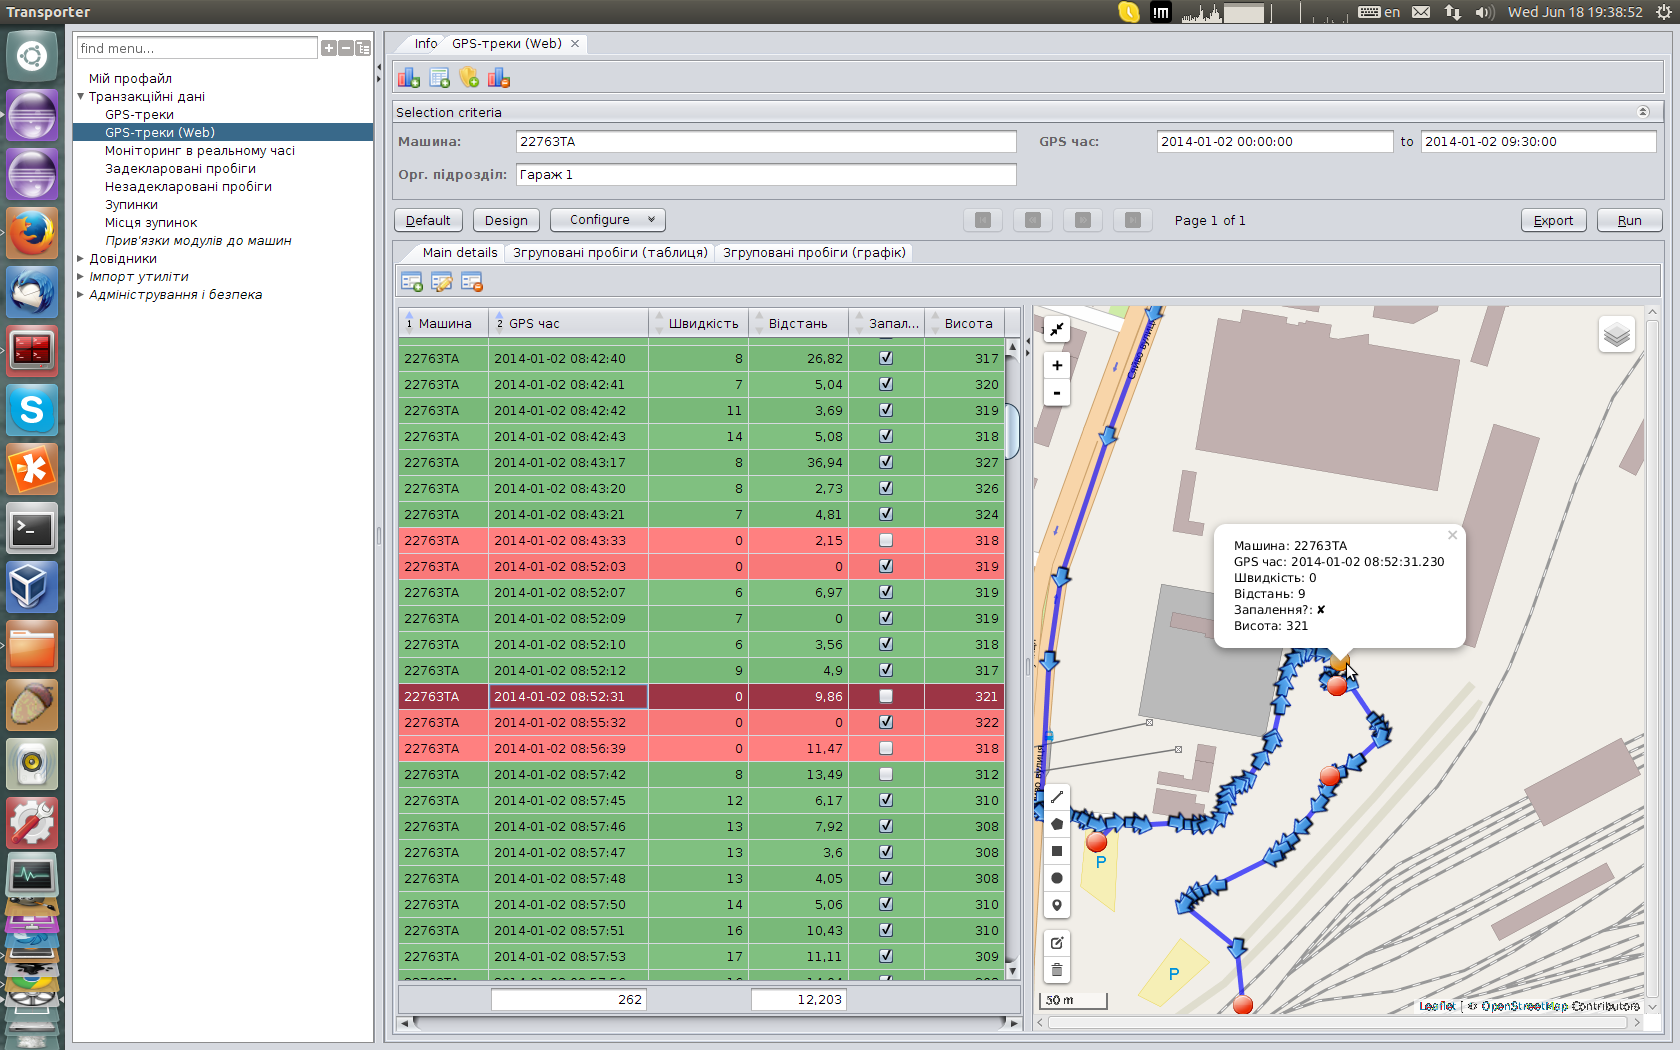
\includegraphics[width=\linewidth]{chapters/02-gpstracks/images/17-selected-stoppage-with-popup.png}
\caption{Selected stoppage message with popup}\label{fig:17}
\end{figure}

\newpage
The ability to show large GPS-tracks has been investigated and the results are shown on figure~\ref{fig:18}. Here the data from one machine for one month has been shown. It includes ~28000 messages and ~1500 kilometers of track movements. The performance is reasonable (at least for desktop browsers and TG java client, android browser client is somewhat slower).

\begin{figure}[H]
\centering
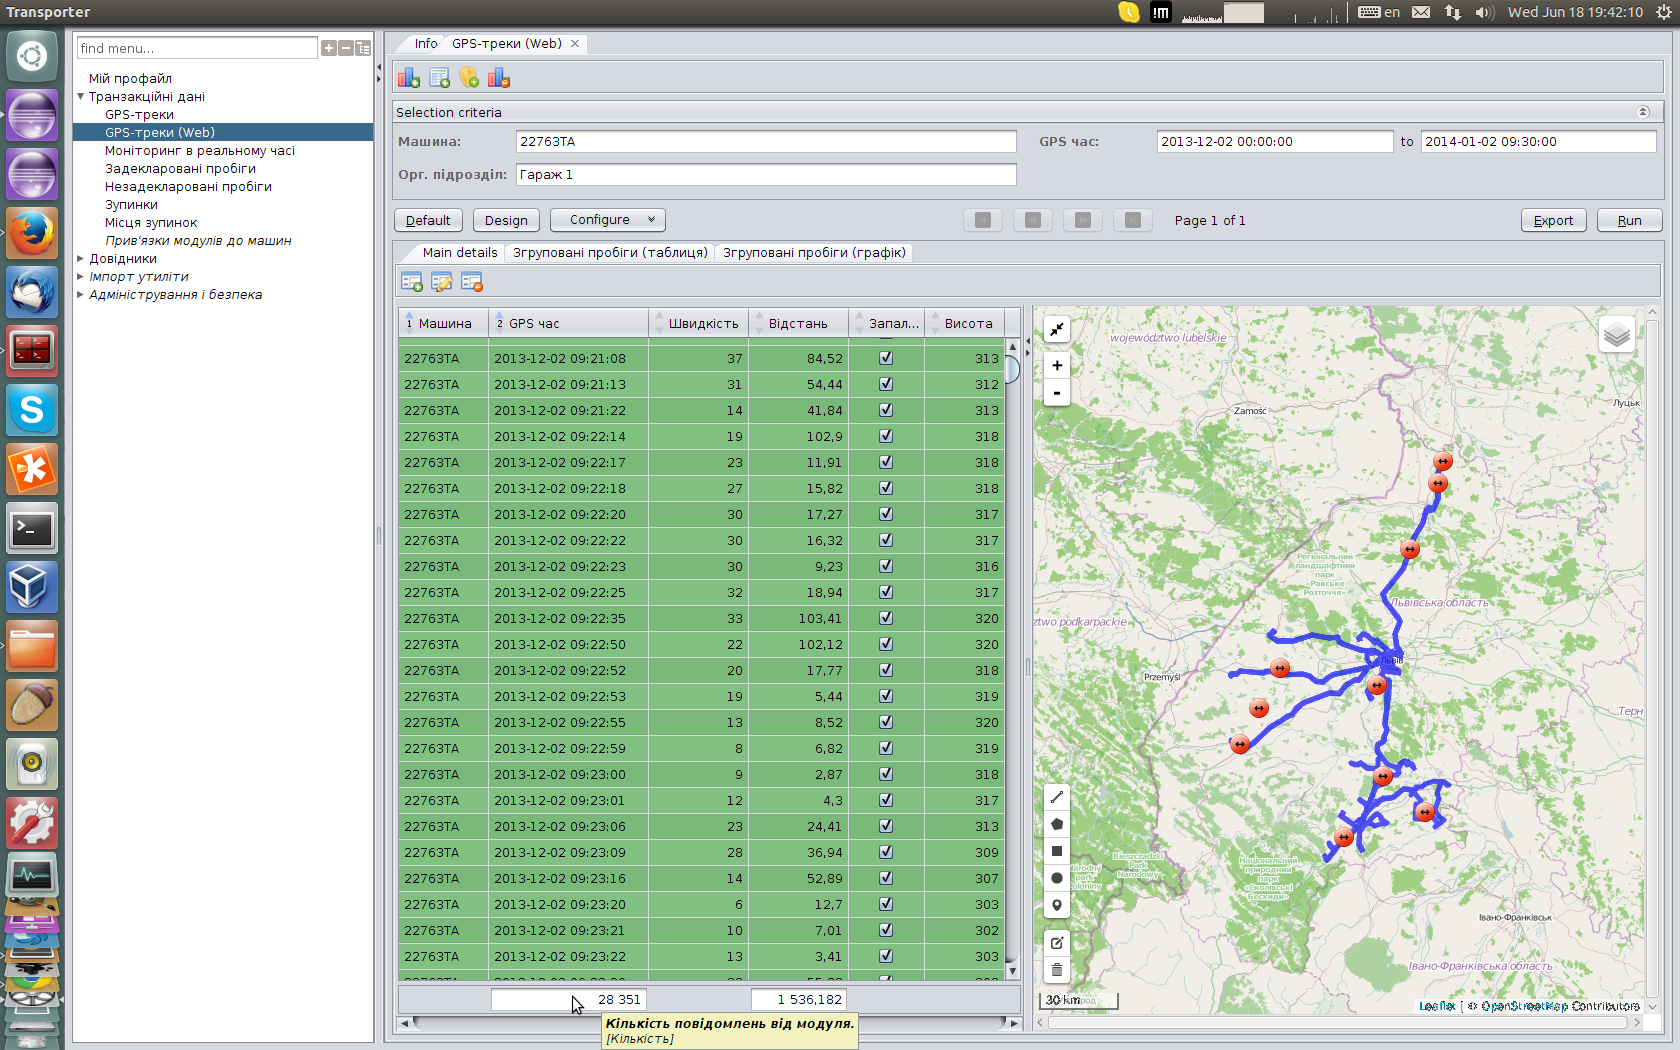
\includegraphics[width=\linewidth]{chapters/02-gpstracks/images/18-huge-dataset-processed-1machine-1month.png}
\caption{Large dataset processed (1 machine for 1 month)}\label{fig:18}
\end{figure}

\newpage
Large dataset details is shown on figure~\ref{fig:19} and figure ~\ref{fig:20}.

\begin{figure}[H]
\centering
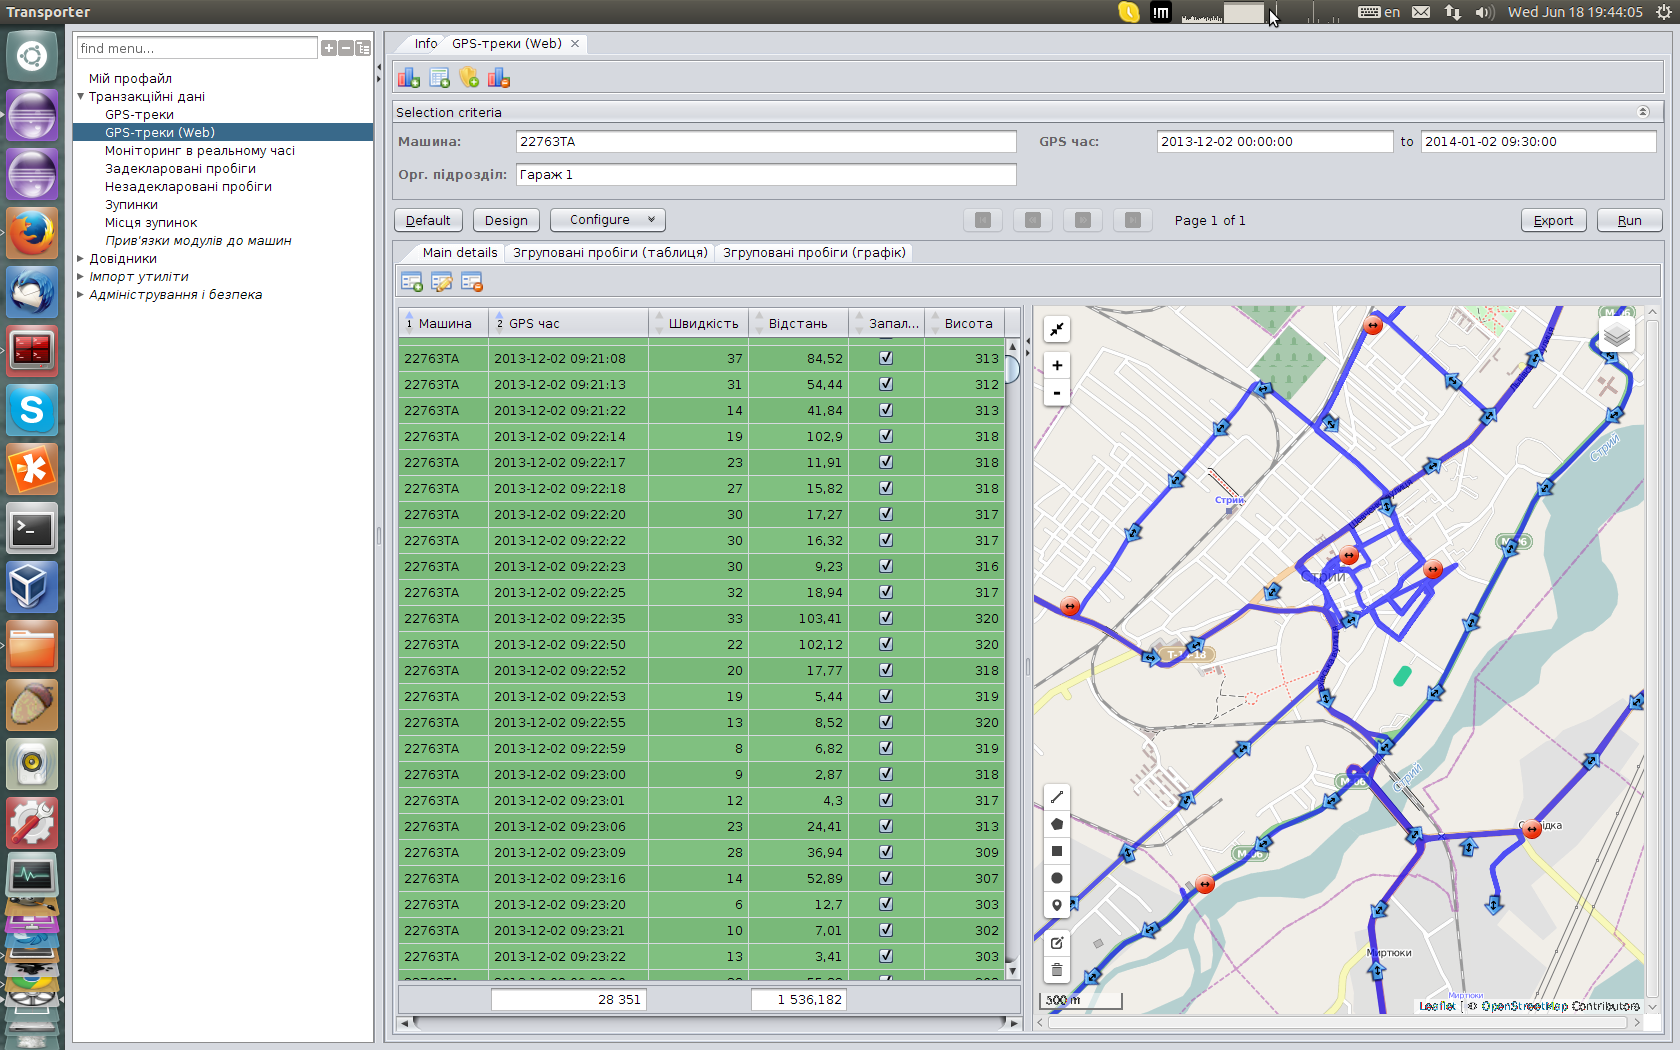
\includegraphics[width=\linewidth]{chapters/02-gpstracks/images/19-middle-details-at-some-place.png}
\caption{Middle details at some place}\label{fig:19}
\end{figure}

\begin{figure}[H]
\centering
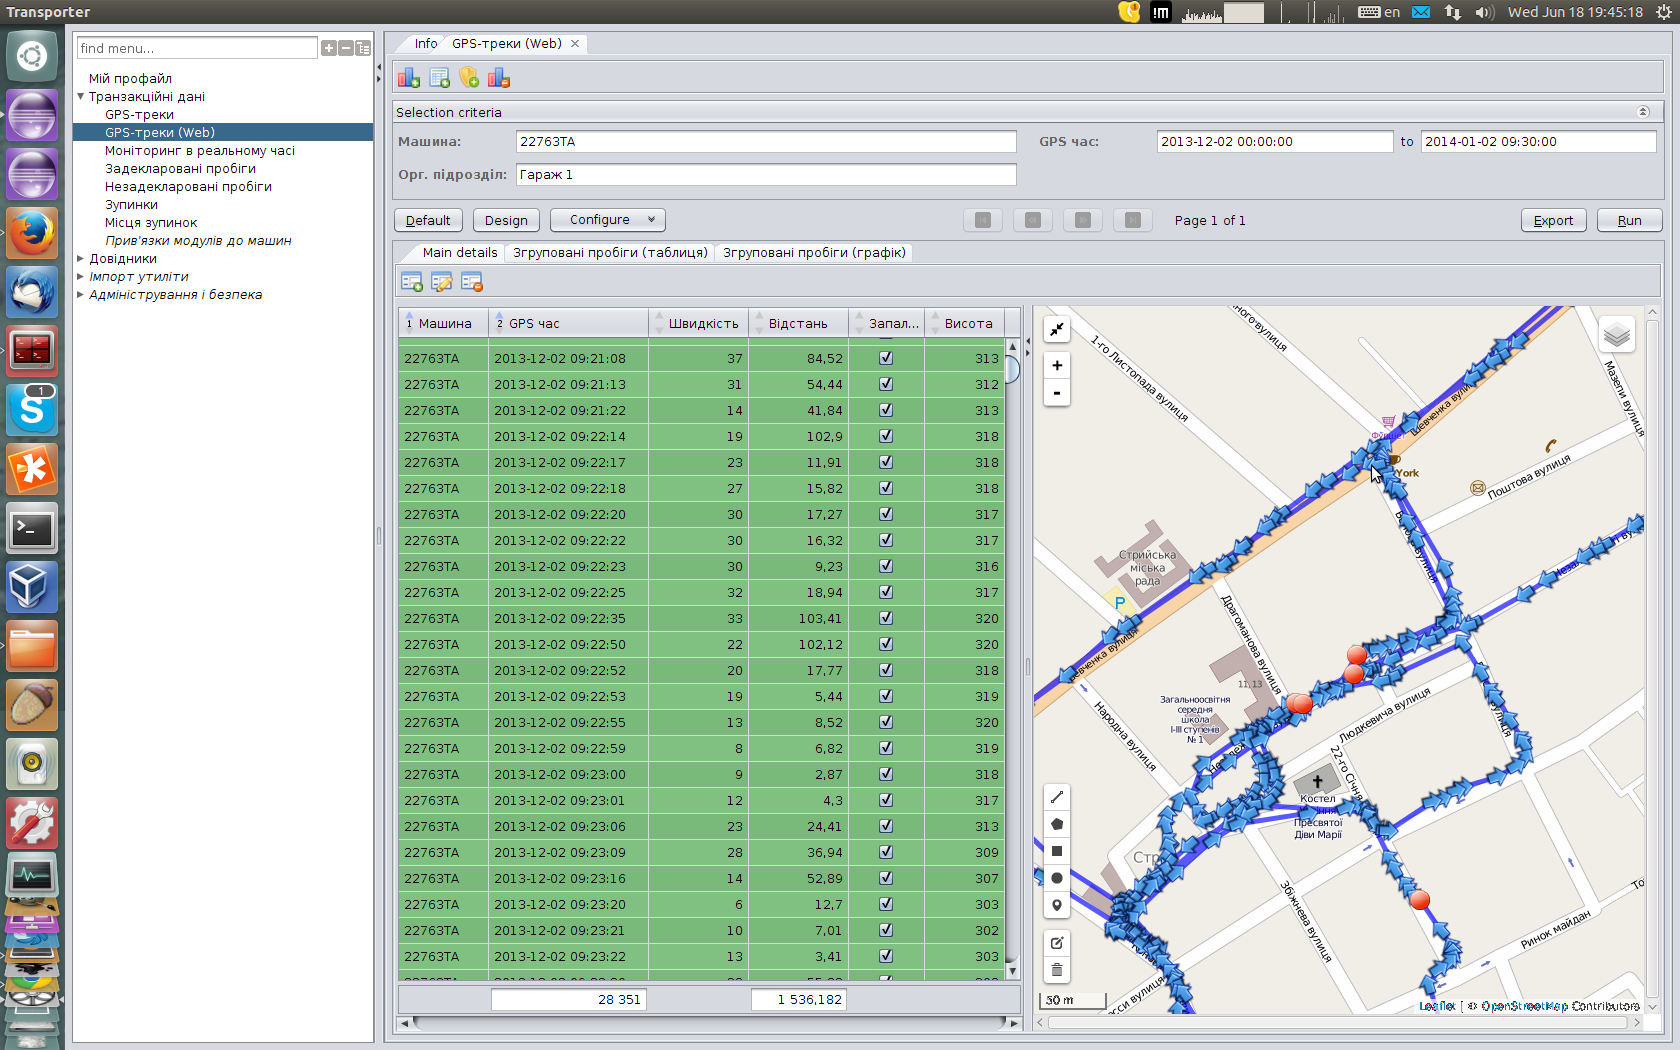
\includegraphics[width=\linewidth]{chapters/02-gpstracks/images/20-full-details-and-marker-hovering-feature.png}
\caption{Full details and marker hovering feature}\label{fig:20}
\end{figure}
  \section{Stoppages}

Stoppages represent ...

\begin{figure}[!htp]
\centering
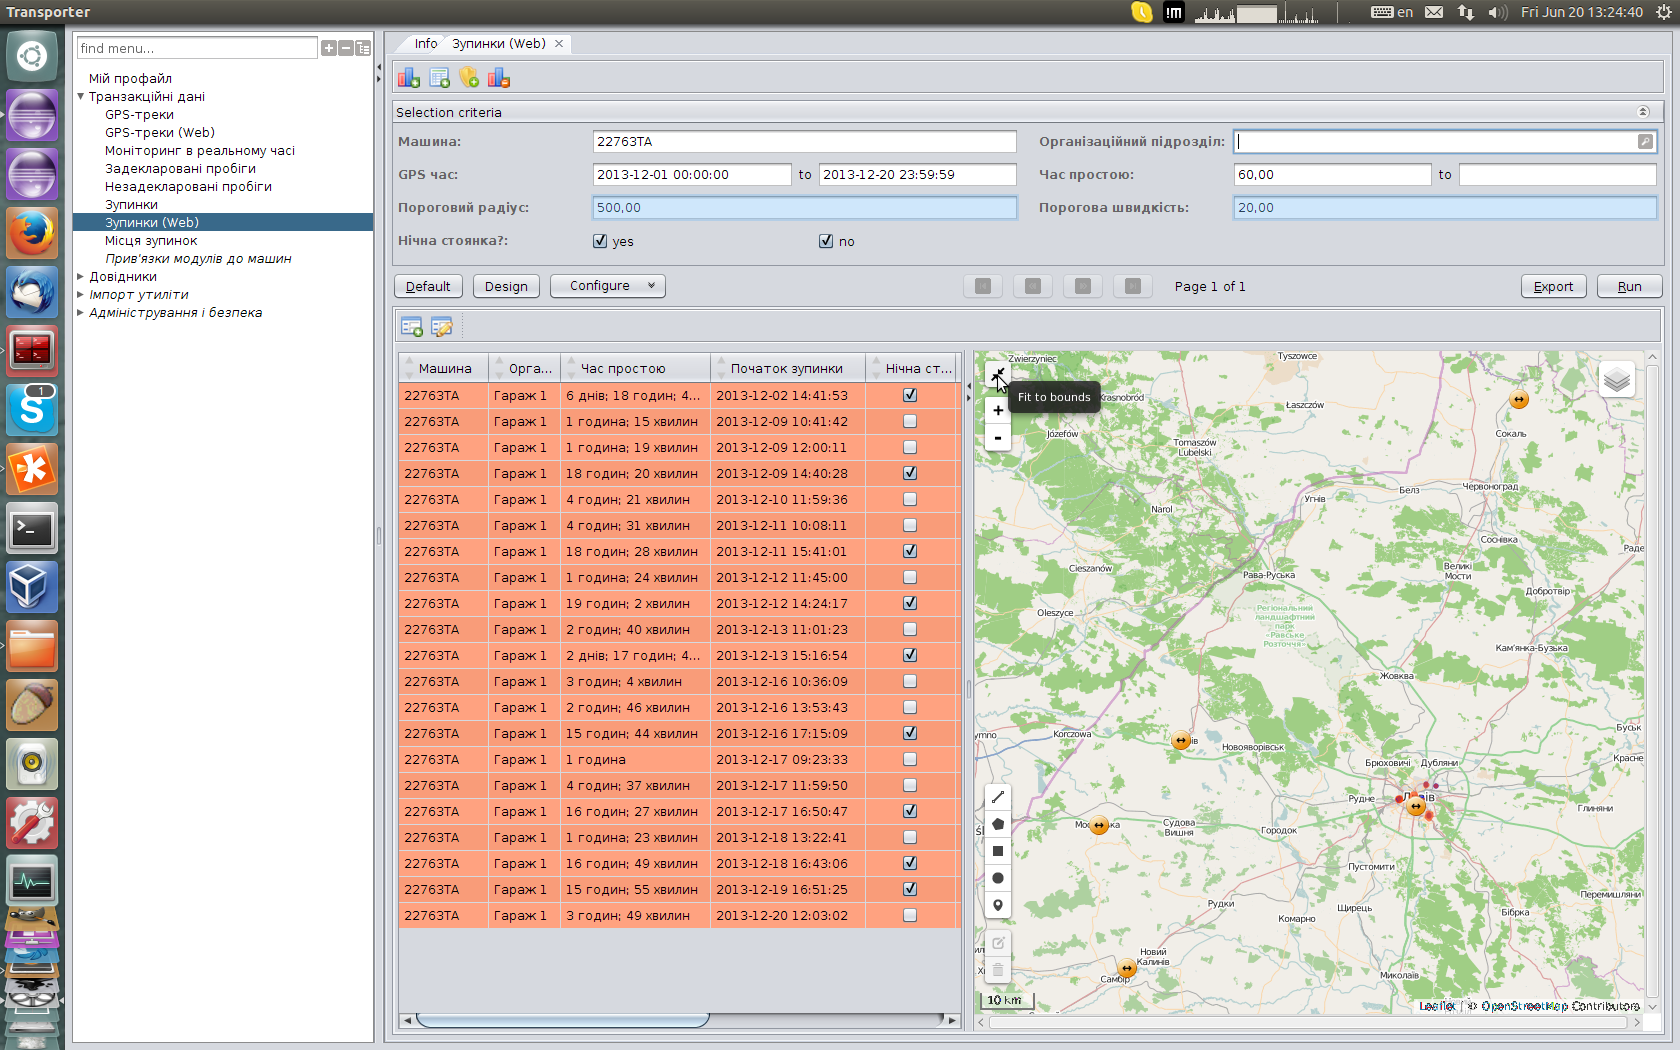
\includegraphics[width=16cm]{chapters/03-stoppages/images/21-all-stoppages-using-fit-to-bounds-button.png}
\caption{all-stoppages-using-fit-to-bounds-button}\label{fig:21}
\end{figure}

\begin{figure}[!htp]
\centering
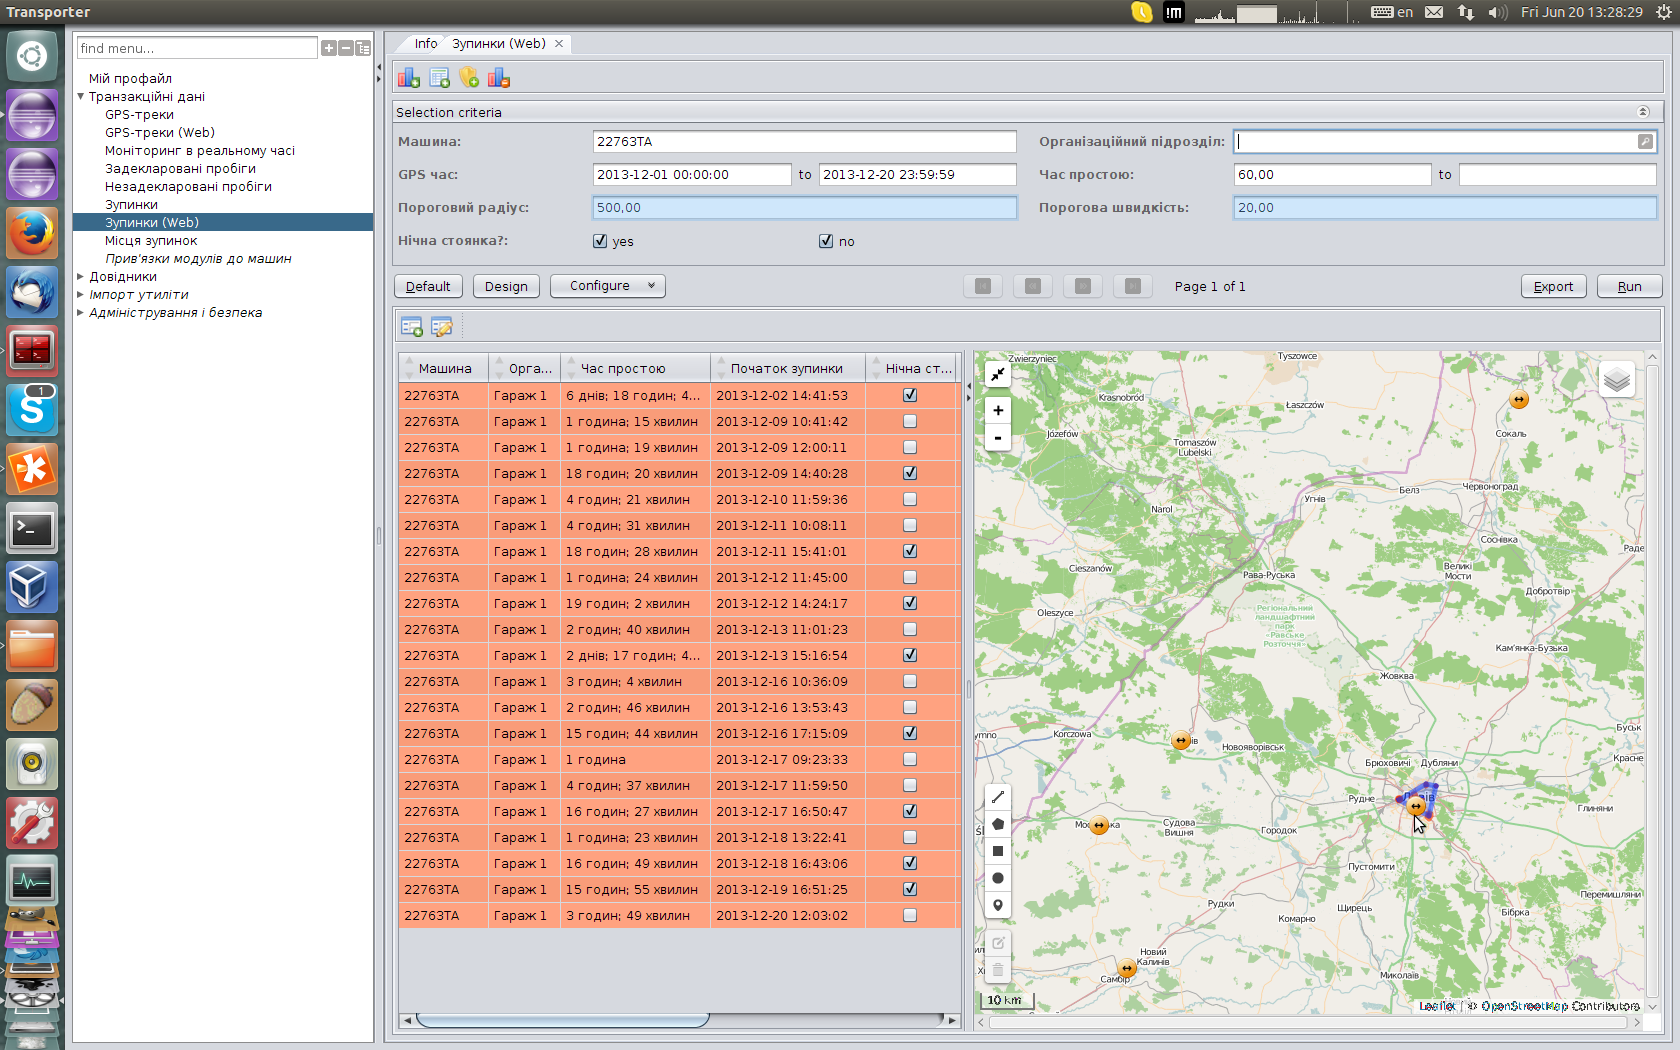
\includegraphics[width=16cm]{chapters/03-stoppages/images/22-part-of-stoppages-zooming-by-clicking-cluster-near-lviv.png}
\caption{part-of-stoppages-zooming-by-clicking-cluster-near-lviv}\label{fig:22}
\end{figure}

\begin{figure}[!htp]
\centering
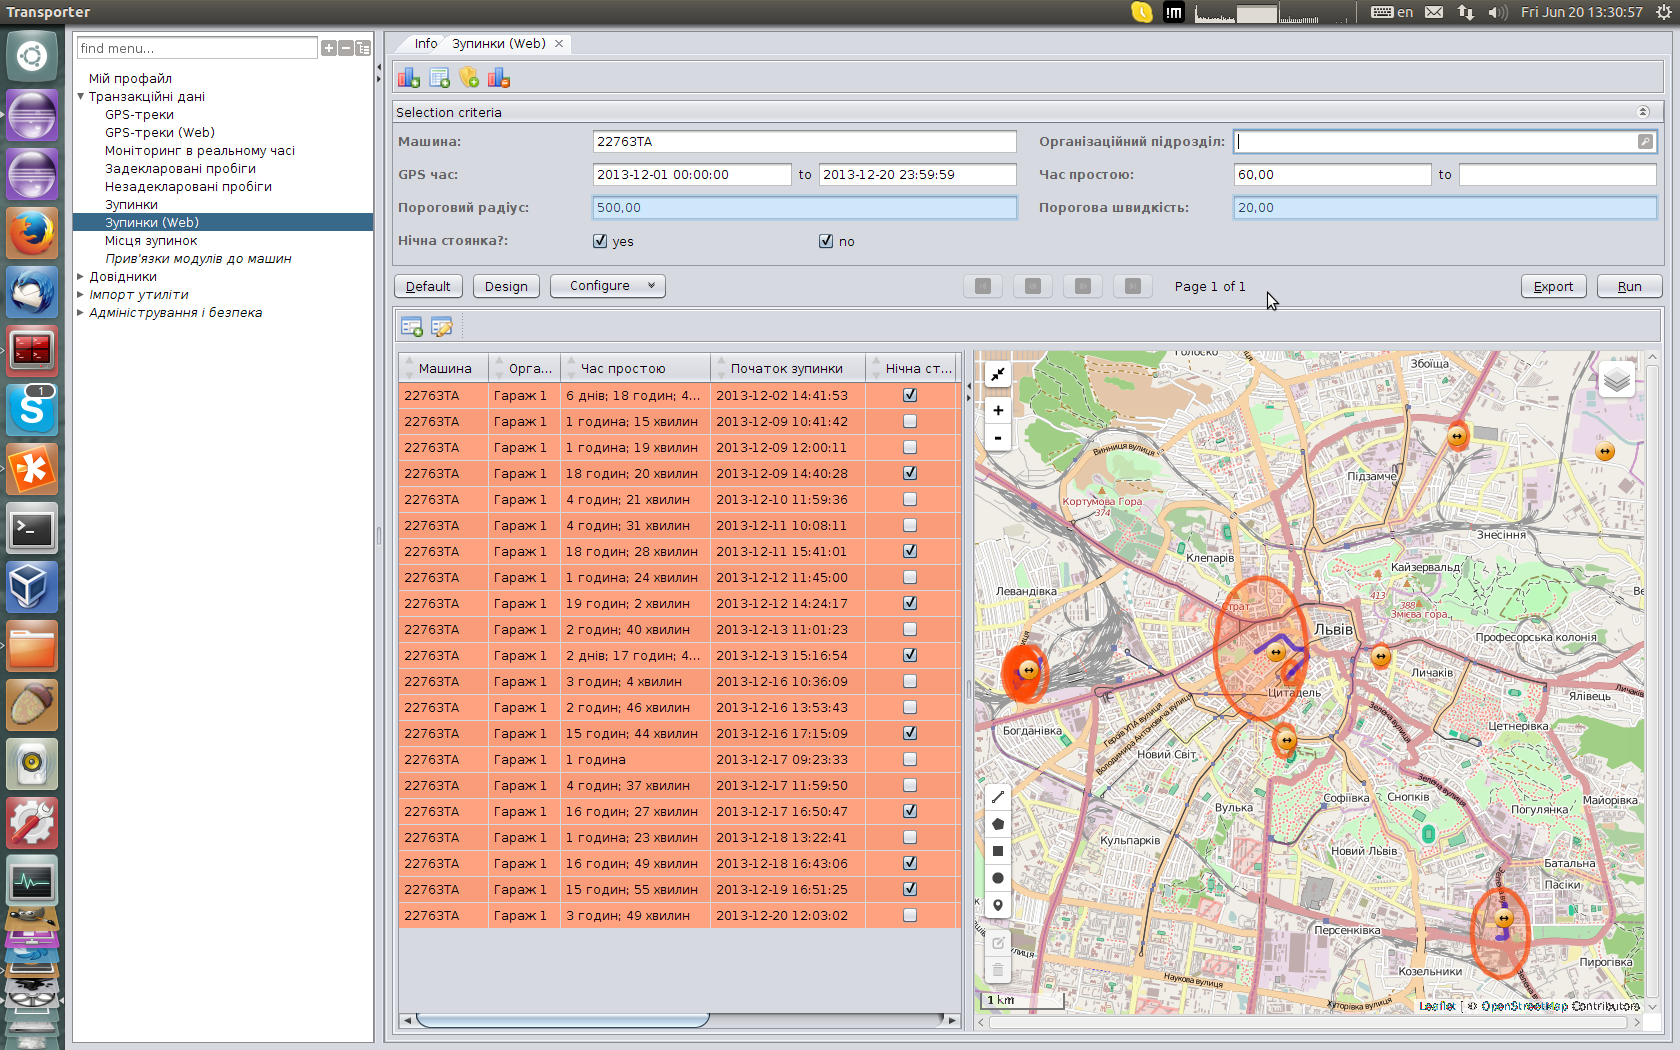
\includegraphics[width=16cm]{chapters/03-stoppages/images/23-part-of-stoppages-zoomed-in.png}
\caption{part-of-stoppages-zoomed-in}\label{fig:23}
\end{figure}

\begin{figure}[!htp]
\centering
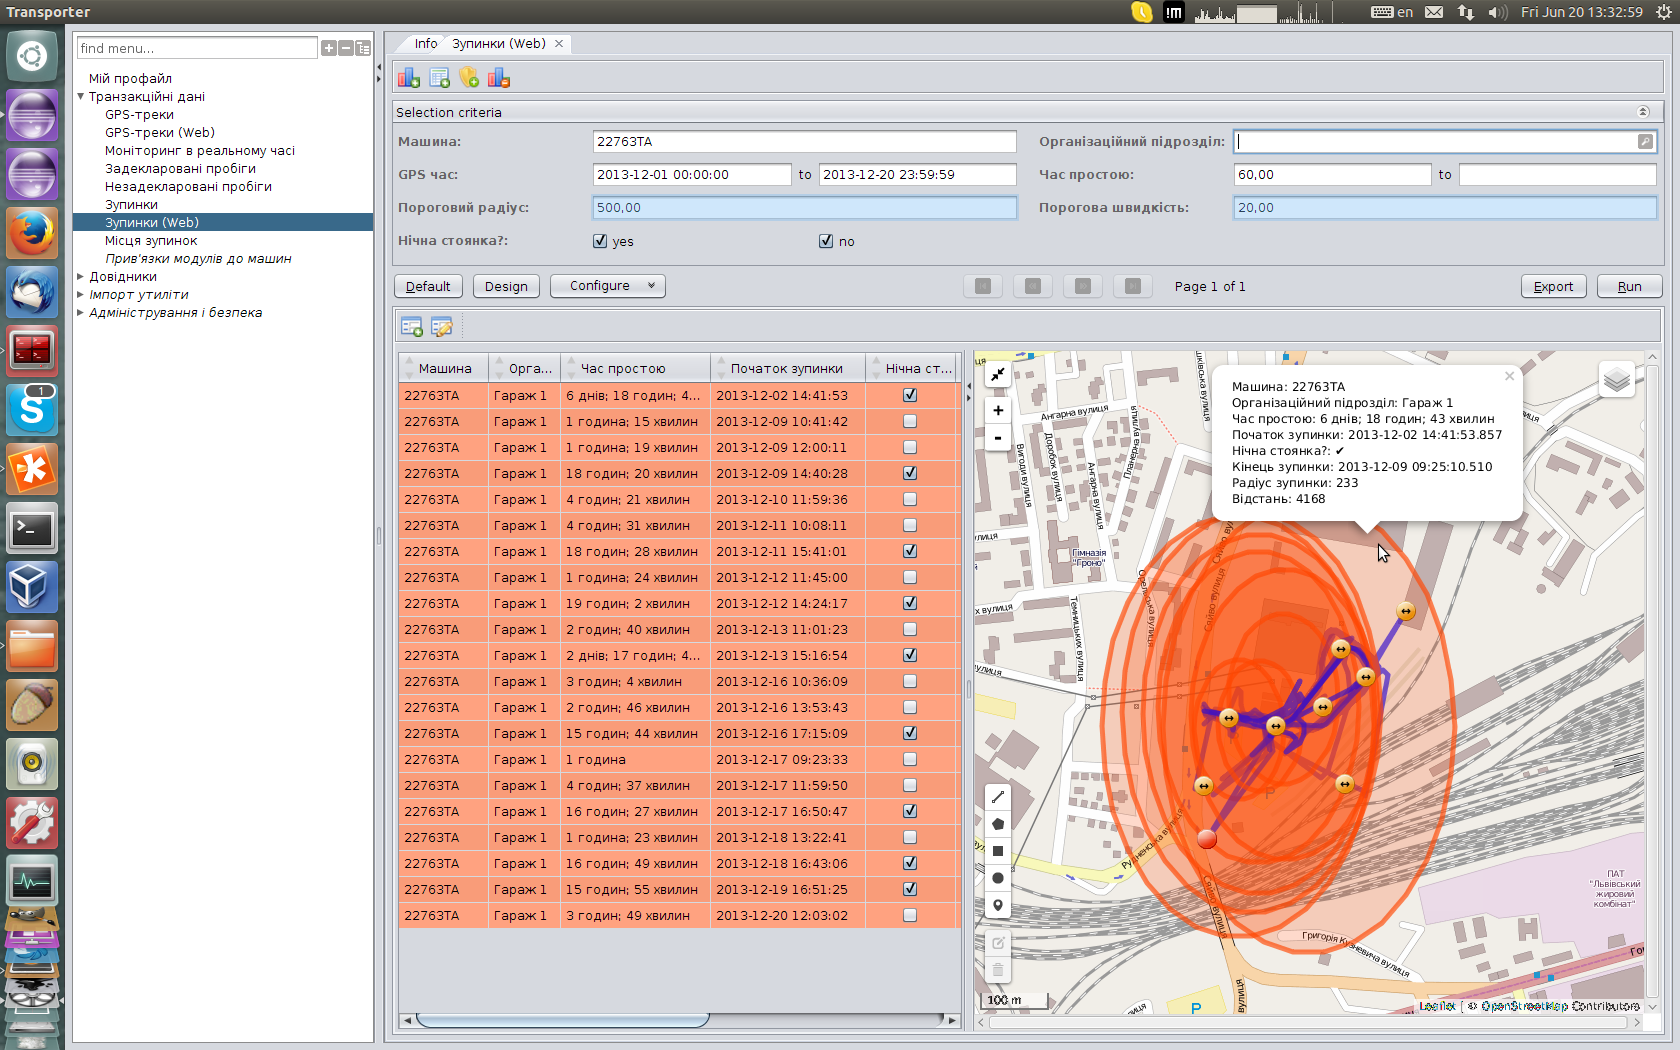
\includegraphics[width=16cm]{chapters/03-stoppages/images/24-a-plenty-of-night-stoppages-in-the-same-place-with-one-selected-popup-details.png}
\caption{a-plenty-of-night-stoppages-in-the-same-place-with-one-selected-popup-details}\label{fig:24}
\end{figure}

\begin{figure}[!htp]
\centering
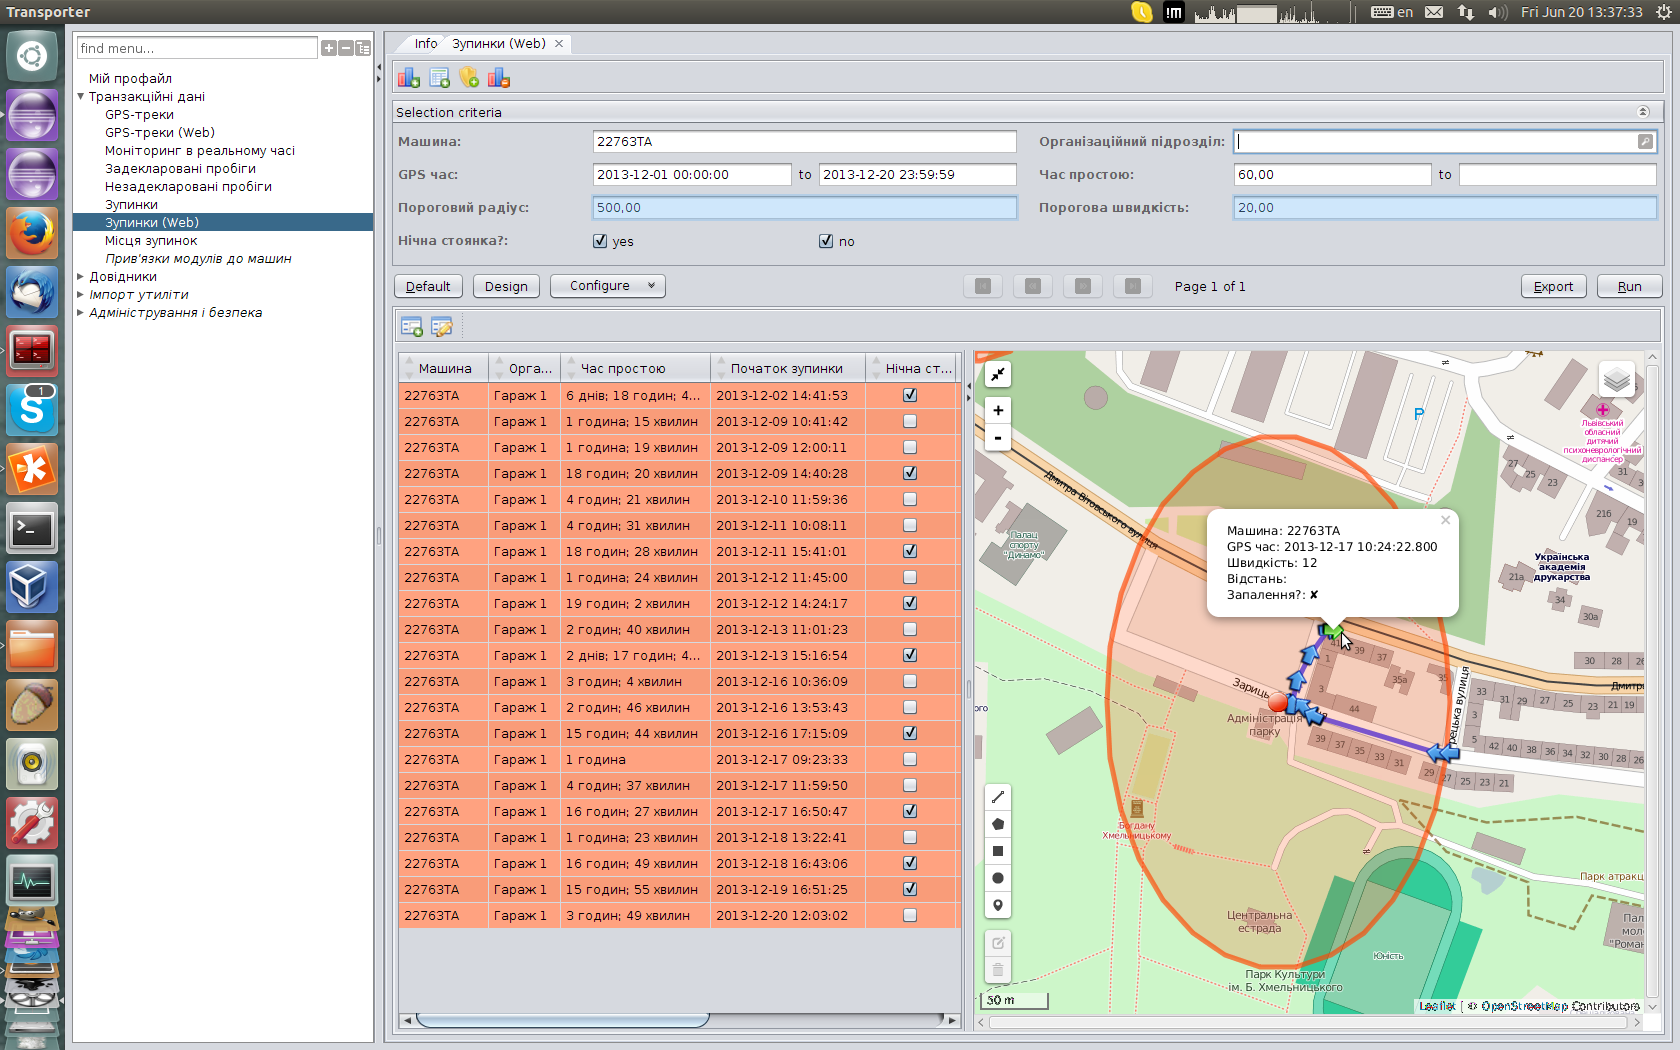
\includegraphics[width=16cm]{chapters/03-stoppages/images/25-detailed-stoppage-analysis-by-its-messages.png}
\caption{25-detailed-stoppage-analysis-by-its-messages}\label{fig:25}
\end{figure}

\begin{figure}[!htp]
\centering
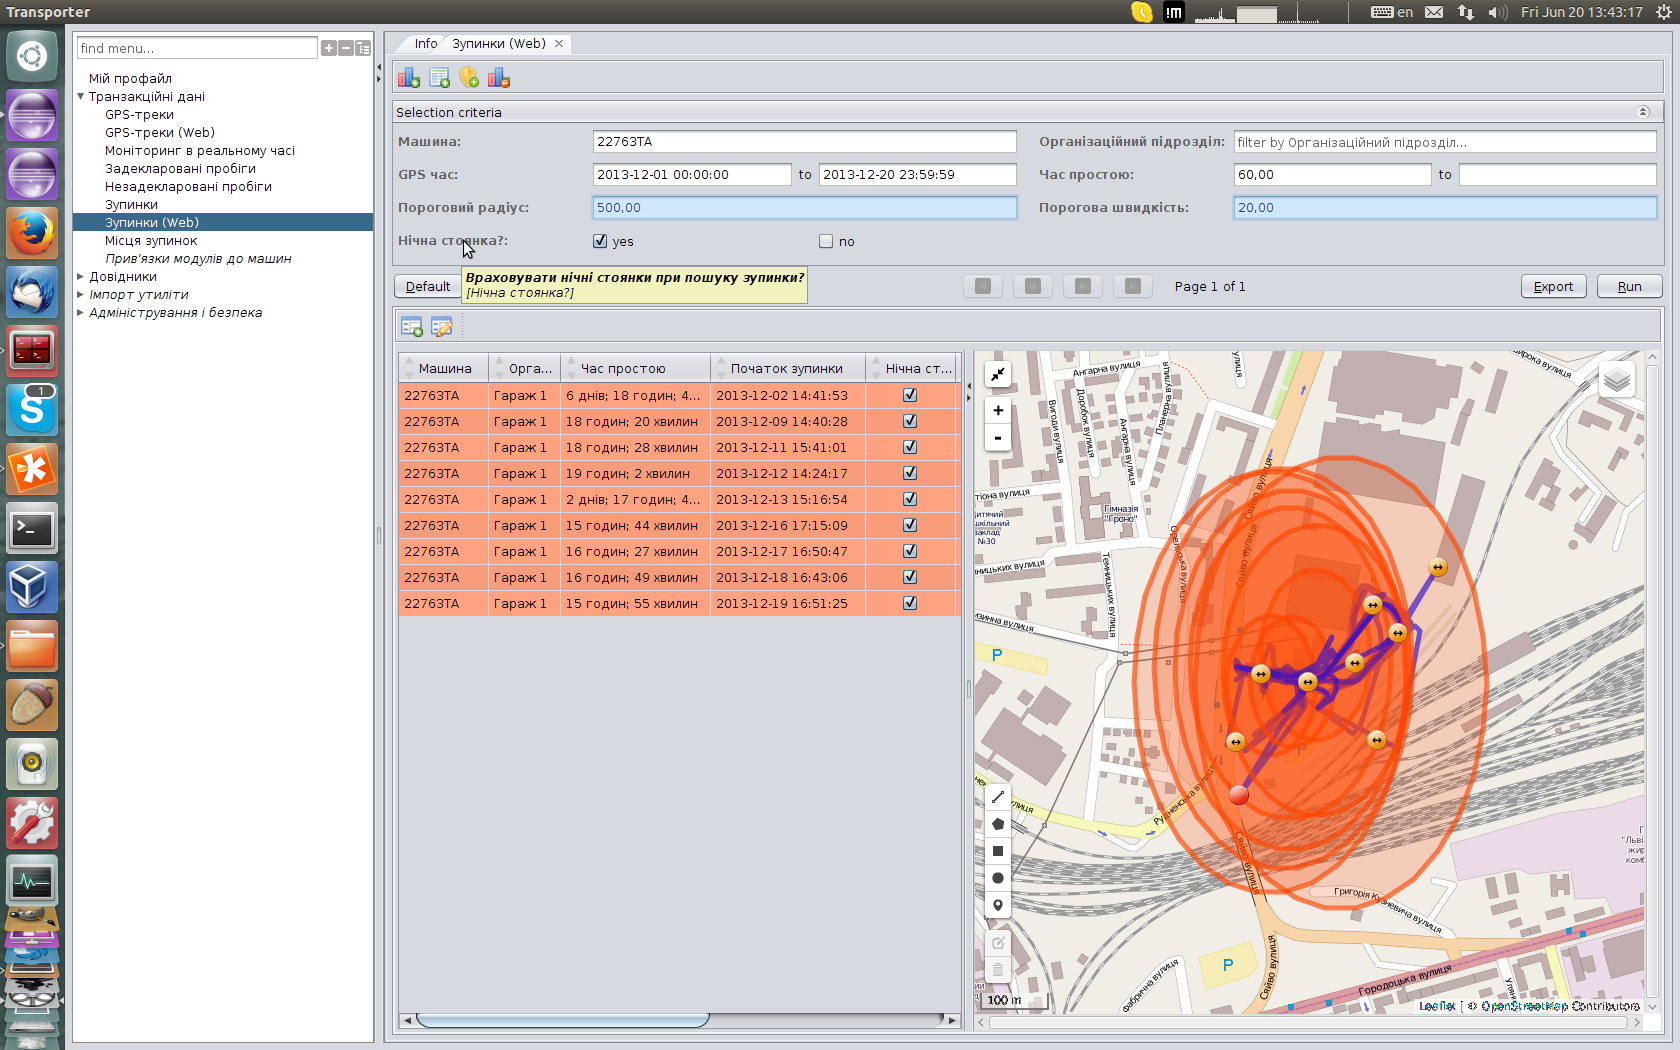
\includegraphics[width=16cm]{chapters/03-stoppages/images/26-determining-whether-machine-has-nightstopped-at-base-in-particular-period-of-time.png}
\caption{determining-whether-machine-has-nightstopped-at-base-in-particular-period-of-time}\label{fig:26}
\end{figure}

\begin{figure}[!htp]
\centering
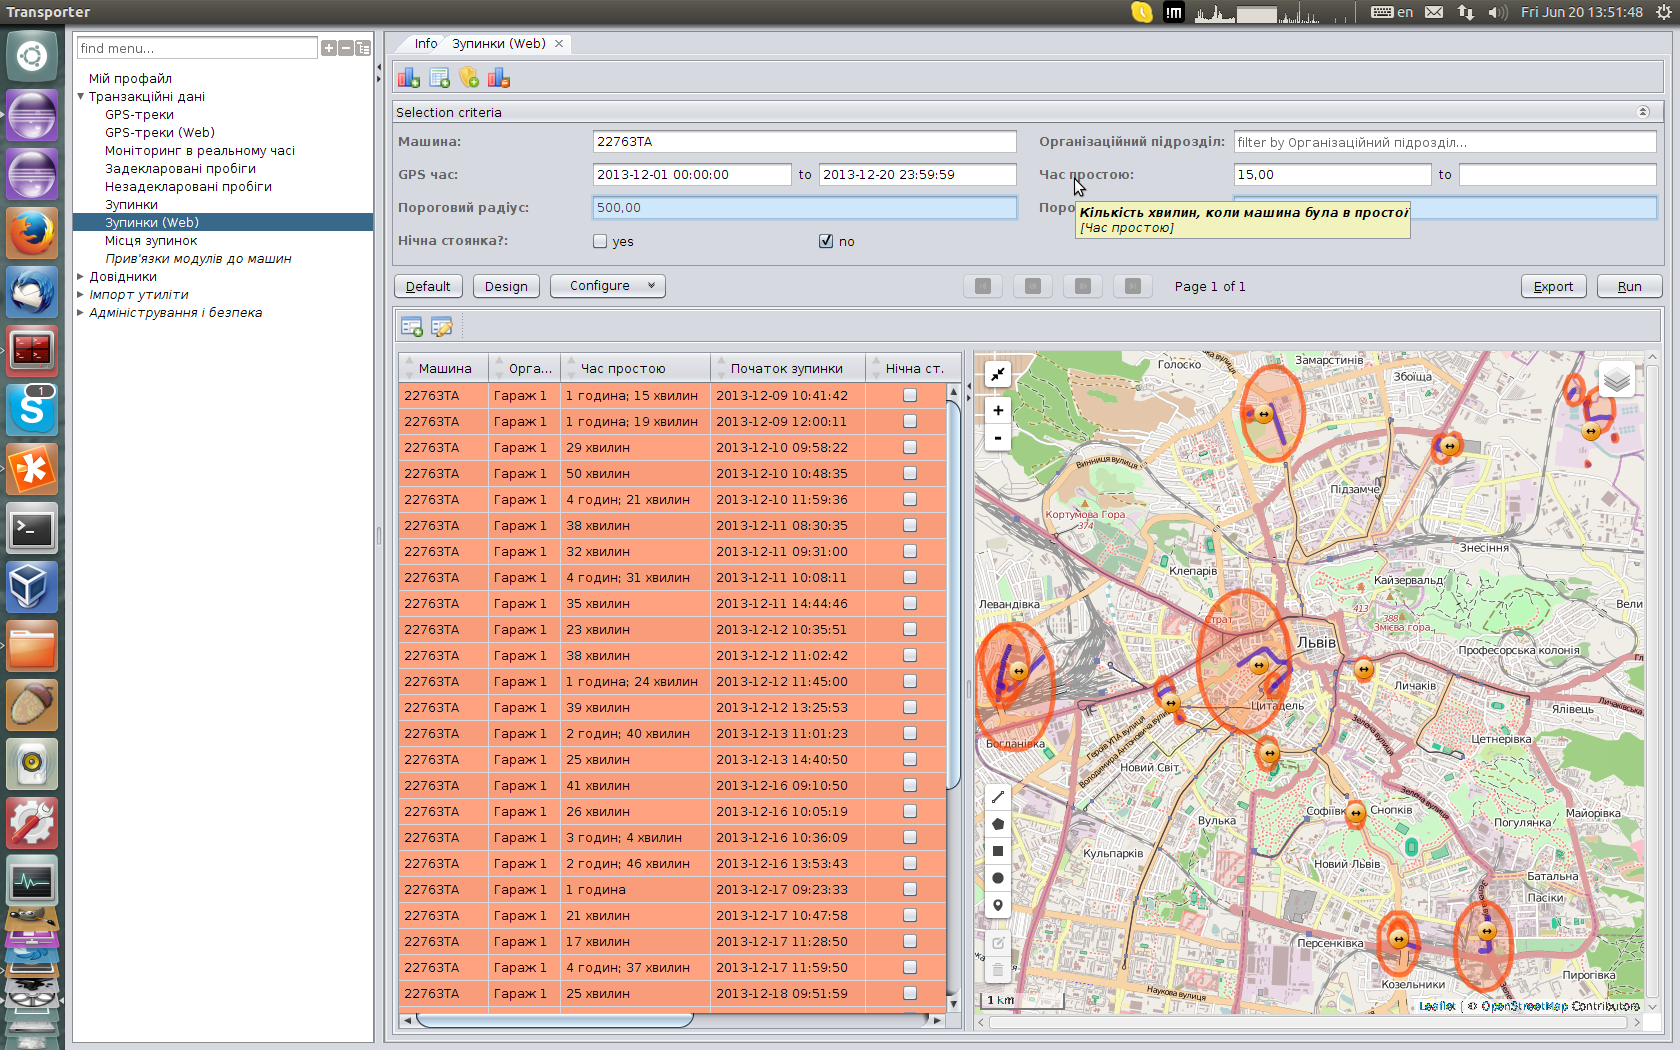
\includegraphics[width=16cm]{chapters/03-stoppages/images/27-determining-stoppages-with-more-than-15-minutes-duration.png}
\caption{determining-stoppages-with-more-than-15-minutes-duration}\label{fig:27}
\end{figure}
\end{document}